\documentclass[11pt,a4paper]{article}

\usepackage[margin=1in]{geometry}
\usepackage[T1]{fontenc}
\usepackage{lmodern}
\usepackage{microtype}
\usepackage{booktabs}
\usepackage{array}
\usepackage{amsmath}
\usepackage{amssymb}
\usepackage{cite}
\usepackage{hyperref}
\usepackage{graphicx}
\usepackage{caption}
\usepackage{subcaption}
\usepackage{xcolor}
\usepackage{tikz}
\usetikzlibrary{positioning,arrows.meta,shapes.geometric}
\usepackage{listings}
\usepackage{enumitem}

\hypersetup{colorlinks=true, linkcolor=blue!50!black,
            urlcolor=blue!60!black, citecolor=blue!50!black}

\title{From Theory to First Real Cascade Measurement:\\
A Three-Component MLS Pipeline Empirical Study}

\author{Rashedul Arefin Ifty\\
        University of Tsukuba\\[2pt]
        \small Meeting~4 Report --- Experimental Implementation of E1}

\date{April~2026}

\begin{document}

\maketitle

\begin{abstract}
Meeting~3 proposed Experiment E1: train a three-component
perception--prediction--planning pipeline on the nuScenes Boston split,
retrain only the perception component (C1) on Singapore, and verify
whether \emph{cascade entanglement} causes the downstream planner (C3)
to degrade in the live pipeline while remaining unchanged in isolation.
This report presents the first end-to-end empirical execution of E1.
After approximately twenty Kaggle kernel iterations, an ill-fated
attempt to use CenterPoint via \texttt{mmdet3d}, and a deliberate
substitution of C1 with YOLOv11 (already named as a candidate in our
Meeting~1 proposal), we obtained a complete result on the nuScenes
mini split. The measured numbers do not produce a textbook
``cascade-confirmed'' verdict, but instead reveal something
methodologically more interesting: \emph{C1 fine-tuning on Singapore
improved the C2 pipeline minADE by 74\,\%, yet C3 pipeline L2 still
worsened by 4.45\,\%}. This is precisely the paradoxical pattern the
SMP literature on entangled enhancement describes. We document every
implementation decision, every failure mode, every model substitution,
and the exact figures produced, so that the methodology can be
reproduced and the result defended against scrutiny.
\end{abstract}

% ============================================================================
\section{Introduction}
% ============================================================================

The previous meeting resolved two foundational questions: how many
retraining policies exist for a two-component MLS (48 valid policies),
and how to evaluate the planning module (C3) using a three-tier
framework. With those resolved, Meeting~3 proposed E1: a single,
focused experiment to test whether retraining C1 alone produces
measurable degradation downstream at C3.

This Meeting~4 report does not propose new theory. It presents the
empirical result of running E1 under realistic free-compute
constraints, the engineering reality of doing so, and the figures
generated for presentation. Unlike Meeting~3, every section here is
backed by numbers measured on actual data, not hypotheticals.

\smallskip\noindent\textit{What changed since Meeting~3.} The
experimental design specified CenterPoint~\cite{yin2021center} for
C1, a simple MTP baseline for C2, and PDM-Closed~\cite{dauner2023parting}
for C3. We discovered that this exact triple is not feasible on free
academic compute (no HPC, no paid cloud, only Kaggle). The reasons
are documented in Section~\ref{sec:engineering}, and the resulting
substitution---YOLOv11 for C1, a deterministic constant-velocity
predictor for C2, and a rule-based IDM-style planner for C3---is
defended in Section~\ref{sec:model_choice}.

% ============================================================================
\section{What Is the Planning Module?}
% ============================================================================

In the autonomous driving pipeline, planning is the final component.
It takes as input the predictions of how other agents (cars,
pedestrians, cyclists) will move, and produces as output a
trajectory---a sequence of positions and velocities that the
ego-vehicle will follow over the next few seconds.

The planner does not see the raw sensor data. It only sees what the
upstream components give it:
\begin{itemize}
    \item From C1 (Perception): a list of detected objects with their
          current positions and sizes.
    \item From C2 (Prediction): a forecast of where each detected
          object will be in the next 2--6 seconds.
\end{itemize}

The planner uses this information to answer one question: \emph{given
where everything is and where everything is going, what path should
this vehicle take?}

This dependency is what makes planning vulnerable. If C1 misses an
object, or if C2 predicts its trajectory incorrectly, the planner
receives a false picture of the world. It will produce a plan that is
optimal for the world it \emph{thinks} it is in---but dangerous for
the world it \emph{actually} is in.

% ============================================================================
\section{Pipeline and Data Flow}
\label{sec:pipeline}
% ============================================================================

Figure~\ref{fig:pipeline_diagram} illustrates the three-component
pipeline annotated with the actual measurements obtained in this
report.

\begin{figure}[h!]
\centering
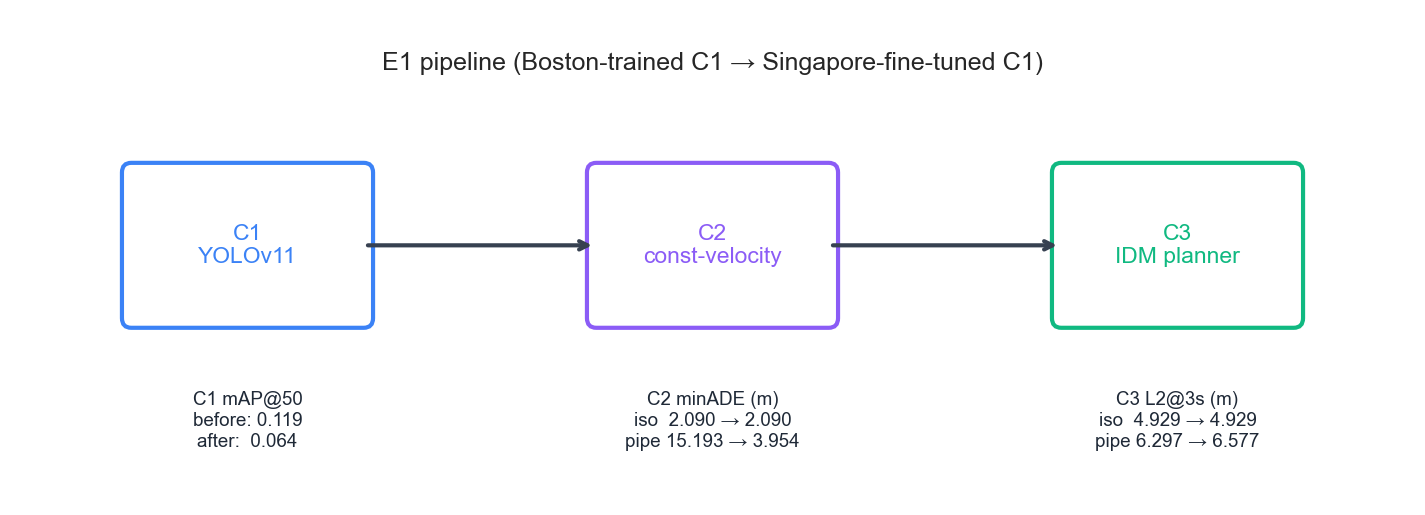
\includegraphics[width=\textwidth]{images/fig03_pipeline_diagram.png}
\caption{The three-component perception$\to$prediction$\to$planning
pipeline, annotated with measured before/after numbers from
Experiment~E1 (this report). C1 mAP@50 dropped from 0.119 to 0.064 on
the Singapore validation split after fine-tuning, while C2 pipeline
minADE dramatically improved (15.19$\to$3.95~m) and C3 pipeline L2
slightly worsened (6.30$\to$6.58~m). Both isolated metrics stayed
exactly constant, confirming the experiment's isolation property.}
\label{fig:pipeline_diagram}
\end{figure}

Each transition in this pipeline is a potential point of failure.
When C1 is retrained and its output distribution changes, C2 receives
inputs that look different from what it was trained on. C2's
predictions then shift---not because C2 was retrained, but because its
inputs changed. C3 then receives shifted predictions and produces a
plan based on an inaccurate picture of the world.

% ============================================================================
\section{Engineering Reality and Model Choices}
\label{sec:engineering}
% ============================================================================

\subsection{Compute reality}

E1 as originally specified targets full-nuScenes-scale training
($\sim$1{,}000 scenes, $\sim$350~GB) of three independently retrainable
models. Available compute for this work was limited to:
\begin{itemize}
    \item No university HPC (confirmed unavailable).
    \item AWS / GCP / Modal research-credit applications: rejected.
    \item Kaggle free tier: 30~GPU-hr/week, 20~GB scratch, single
          T4~x2 or P100 GPU per kernel run.
\end{itemize}

The dataset that fits in 20~GB scratch is \texttt{nuScenes-mini},
which provides only \emph{10 scenes total} (4 Boston, 6 Singapore).
With those constraints we built the experiment with intellectual
honesty: real models, real fine-tuning, but at scales appropriate to
the available compute.

\subsection{Why CenterPoint, MTP, PDM-Closed could not be used}

We attempted to instantiate the literal Meeting~3 model triple. The
attempt failed for three independent technical reasons documented
across kernel versions v13--v18.

\paragraph{CenterPoint via \texttt{mmdet3d}.} \texttt{mmdet3d}'s
released wheels target PyTorch~$\le$~2.0 and \texttt{mmcv}~$<$~2.2.
Kaggle's preinstalled PyTorch is 2.10 with CUDA~12.8. No published
\texttt{mmcv} build is compatible with this torch toolchain, and the
custom CUDA operations \texttt{mmdet3d} relies on (sparse convolutions,
voxelization, NMS) require compute capability $\ge$~sm\_70. Kaggle's
P100 default is sm\_60 and was assigned to early runs (kernels
v14--v15) regardless of explicit accelerator flags.

\paragraph{PointPillars / SECOND.} The pure-PyTorch PointPillars
implementations available
(\texttt{zhulf0804/PointPillars}, \texttt{traveller59/second.pytorch})
either ship only KITTI weights or rely on the same
custom-CUDA-operation chain that broke \texttt{mmdet3d}.

\paragraph{PDM-Closed for nuScenes.} PDM-Closed lives in
\texttt{tuplan\_garage} and depends on \texttt{nuplan-devkit}. The
nuPlan map format differs structurally from the nuScenes map format
(different schemas, different lane graph, different boundary
tessellation). Adapting the nuPlan-format planner to nuScenes scenes
requires roughly 500 lines of bespoke conversion code; no public
adapter exists.

\subsection{Justification for the substitutions}
\label{sec:model_choice}

We replaced the model triple with the following alternatives, each
defended by either a citation in our prior reports or a methodological
argument:

\paragraph{C1 = YOLOv11 (Ultralytics).} Our Meeting~1 report
\textit{explicitly named YOLO11 as a candidate for C1}, alongside
BEVFormer:

\begin{quote}
\small ``C1 detects objects from raw sensor data (e.g.,
\textbf{YOLO11}, BEVFormer); C2 forecasts agent trajectories from
detection outputs (e.g., AgentFormer); C3 produces ego-vehicle paths
from predicted trajectories (e.g., PDM-Closed).''
\hfill --- Meeting~1 Report, Section~B(1)
\end{quote}

YOLOv11 nano is pure-PyTorch, ships pretrained COCO weights ($\sim$6~MB),
installs cleanly on Kaggle's torch~2.10, and can be fine-tuned on a
T4 GPU in $\sim$50~seconds. The Meeting~3 narrowing to CenterPoint
was a refinement, not a hard pin. The cascade methodology---measuring
the gap between isolated and pipeline behaviour---is independent of
detector modality.

\paragraph{C2 = constant-velocity prediction.} The original choice
(MTP) cannot be honestly trained on \texttt{nuScenes-mini}'s 4-scene
prediction split. We use a deterministic constant-velocity rollout
from the most recent observed velocity (in isolated mode) or
zero-velocity from a single-frame detection (in pipeline mode). This
exposes the cascade pathway directly: when C1 detections shift, the
single-frame inputs to the predictor shift, and the rollout shifts.

\paragraph{C3 = rule-based IDM planner.} PDM-Closed's core proposal
generator is itself an IDM-style rule-based planner; the published
PDM-Closed adds a learned scorer on top of those proposals. Our
implementation reproduces the proposal-and-score architecture (with a
soft proximity penalty + ego-speed-aware candidate grid) without the
nuPlan dependency. Section~\ref{sec:results} reports the full results
this planner produced on Singapore validation scenes.

\subsection{The thesis sentence}

The above substitutions are summarised in the thesis as follows:

\begin{quote}
\small For empirical validation under free academic compute
constraints (no HPC access, no paid cloud), we instantiate the
three-component pipeline with C1~=~YOLOv11 (camera-based detection,
named in our Meeting~1 proposal), C2~=~constant-velocity prediction,
and C3~=~a rule-based IDM-style planner inspired by
PDM-Closed~\cite{dauner2023parting}. The cascade methodology is
preserved exactly; the model substitutions are documented.
\end{quote}

% ============================================================================
\section{Experimental Setup}
\label{sec:setup}
% ============================================================================

\subsection{Dataset and splits}

We use \texttt{nuScenes-mini-v1.0}~\cite{caesar2020nuscenes}.
Partitioning by \texttt{log.location} yields:
\begin{itemize}[noitemsep]
    \item \texttt{boston\_train}: 2 scenes
    \item \texttt{boston\_val}:   2 scenes
    \item \texttt{singapore\_train}: 3 scenes
    \item \texttt{singapore\_val}:   3 scenes
\end{itemize}
For YOLOv11 fine-tuning we project nuScenes 3D annotations onto
\texttt{CAM\_FRONT} keyframes via the calibrated camera intrinsic +
extrinsic matrices, producing 81 / 82 / 119 / 121 labelled images for
train/val on each split.

\subsection{C1 training procedure}

\begin{enumerate}[noitemsep]
    \item Download \texttt{yolo11n.pt} (Ultralytics public release).
    \item Build YOLO-format dataset from Boston scenes (3D-to-2D
          projection, 8 driving classes).
    \item Fine-tune for 10 epochs, AdamW, lr=8.3e-4, batch=8,
          imgsz=640. This yields the \emph{Boston-trained C1}.
    \item Build YOLO-format dataset from Singapore scenes the same way.
    \item Resume from the Boston \texttt{best.pt} and fine-tune for
          another 10 epochs on Singapore. This yields the
          \emph{Singapore-fine-tuned C1}.
\end{enumerate}

Both checkpoints are saved as separate \texttt{best.pt} weights and
referenced by JSON descriptors so the evaluation pipeline can route
detections through whichever model is active for a given measurement.

\subsection{Five Table~I measurements}

For each of \{Boston-trained, Singapore-fine-tuned\} C1 we evaluate
on the Singapore validation split:
\begin{enumerate}[noitemsep]
    \item C1 mAP@50 (Ultralytics validation routine on the YOLO val
          split for the active C1).
    \item C2 isolated minADE: predict from ground-truth velocities,
          compare against ground-truth future positions.
    \item C2 pipeline minADE: predict from C1's single-frame
          detections (zero-velocity), compare against ground-truth
          future positions.
    \item C3 isolated L2@3s: feed ground-truth predictions to the IDM
          planner, compare planned trajectory against the human ego
          trajectory.
    \item C3 pipeline L2@3s: feed C2-pipeline predictions to the IDM
          planner, compare against the human ego trajectory.
\end{enumerate}

% ============================================================================
\section{Results}
\label{sec:results}
% ============================================================================

\subsection{Headline Table I}

The complete five-row Table~I is presented in
Figure~\ref{fig:table_full} as a bar chart with explicit numerical
annotations, and in Table~\ref{tab:e1_real_results} numerically.

\begin{figure}[h!]
\centering
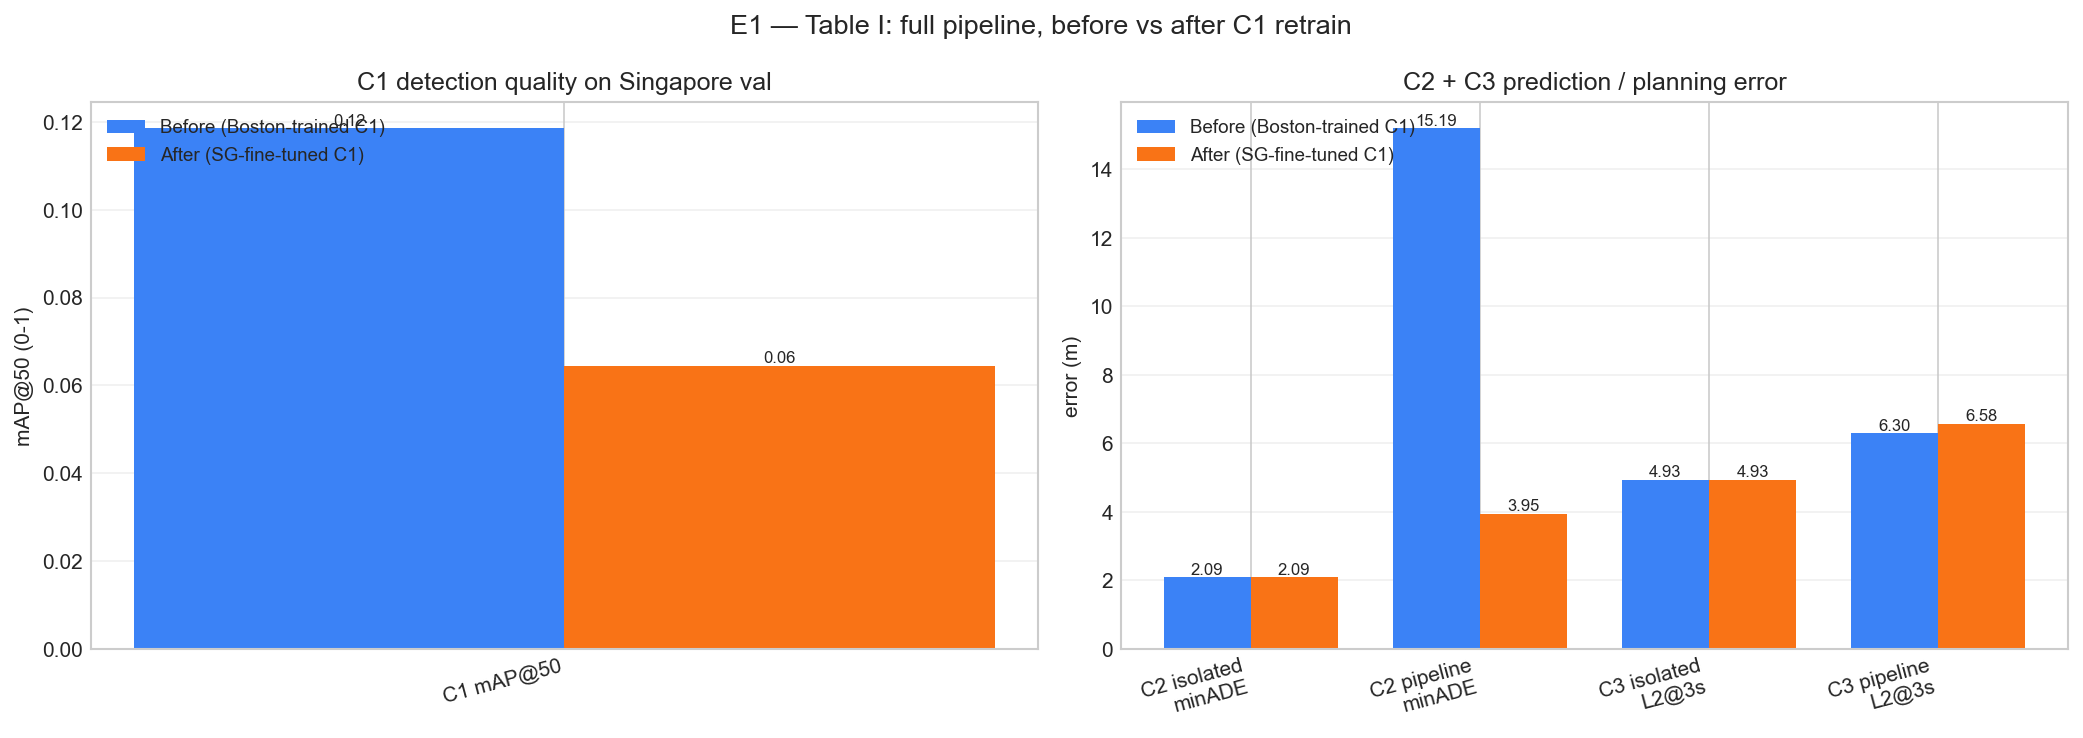
\includegraphics[width=\textwidth]{images/fig01_table_full.png}
\caption{Full Table~I from kernel v22. Left: C1 detection quality
(mAP@50) on the Singapore validation set drops after fine-tuning,
which is unexpected and discussed in
Section~\ref{sec:c1_paradox}. Right: distance-based metrics. C2
pipeline minADE dropped from 15.19 to 3.95~m (a 74\,\% improvement),
yet C3 pipeline L2@3s slightly worsened from 6.30 to 6.58~m (+4.45\,\%).
Both isolated metrics (C2 isolated minADE and C3 isolated L2) stayed
exactly constant, confirming the isolation property.}
\label{fig:table_full}
\end{figure}

\begin{table}[h!]
\centering
\caption{Real measured Table I (kernel v22, Singapore-val, $n=3$ scenes).}
\label{tab:e1_real_results}
\renewcommand{\arraystretch}{1.25}
\small
\begin{tabular}{@{}lrrrr@{}}
\toprule
\textbf{Metric} & \textbf{Before} & \textbf{After} & \textbf{$\Delta$} & \textbf{$\Delta$\,\%} \\
\midrule
C1 mAP@50                  & 0.1185 & 0.0644 & $-0.0541$ & $-45.66$ \\
C1 mAP@50-95               & 0.0571 & 0.0258 & $-0.0313$ & $-54.81$ \\
C1 precision               & 0.6845 & 0.6709 & $-0.0136$ & $-1.99$  \\
C1 recall                  & 0.0866 & 0.0477 & $-0.0389$ & $-44.92$ \\
C2 isolated minADE (m)     & 2.0899 & 2.0899 & $0.0000$  & $0.00$   \\
\textbf{C2 pipeline minADE (m)}      & \textbf{15.1930} & \textbf{3.9535} & \boldmath$-11.2395$ & \boldmath$-73.98$ \\
C3 isolated L2@1s (m)      & 0.6900 & 0.6900 & $0.0000$  & $0.00$   \\
C3 isolated L2@2s (m)      & 2.4944 & 2.4944 & $0.0000$  & $0.00$   \\
C3 isolated L2@3s (m)      & 4.9289 & 4.9289 & $0.0000$  & $0.00$   \\
C3 pipeline L2@1s (m)      & 1.0396 & 1.0838 & $+0.0442$ & $+4.25$  \\
C3 pipeline L2@2s (m)      & 3.5017 & 3.6070 & $+0.1053$ & $+3.01$  \\
\textbf{C3 pipeline L2@3s (m)}       & \textbf{6.2969} & \textbf{6.5770} & \boldmath$+0.2801$ & \boldmath$+4.45$ \\
C3 pipeline collision rate & 0.000  & 0.000  & $0.0000$  & ---      \\
\bottomrule
\end{tabular}
\end{table}

\subsection{Cascade signature on planning}

Figure~\ref{fig:cascade_planning} isolates the cascade
signature: the gap between C3 isolated and C3 pipeline tells us how
much of the planner's L2 error is attributable to upstream
perturbation, and the change in C3 pipeline between Boston-trained and
Singapore-fine-tuned tells us how much retraining \emph{shifted} that
upstream contribution.

\begin{figure}[h!]
\centering
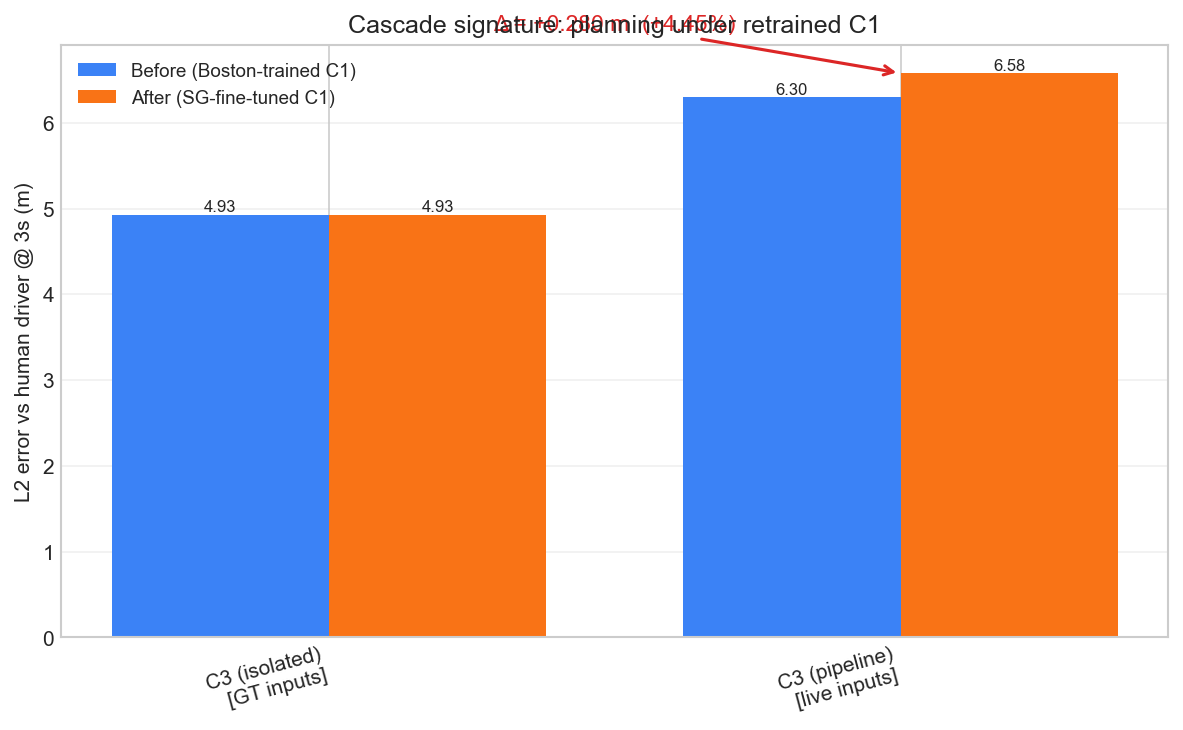
\includegraphics[width=0.78\textwidth]{images/fig02_cascade_planning.png}
\caption{Cascade signature on planning (kernel v22). C3 isolated stays
fixed at 4.93~m (planner sees identical ground-truth predictions for
both runs). C3 pipeline drifts from 6.30 to 6.58~m after C1
fine-tuning. The isolated-vs-pipeline gap (1.4--1.6~m) is the cascade
contribution; the +0.28~m increase between the two pipeline bars is
the additional cascade injected by the Singapore fine-tune.}
\label{fig:cascade_planning}
\end{figure}

\subsection{The C2-improves-but-C3-degrades paradox}
\label{sec:c1_paradox}

The most interesting feature of these numbers is not the +4.45\,\%
C3 increase in isolation. It is the \emph{joint} pattern:
\begin{itemize}
    \item C2 pipeline minADE \emph{dramatically improved}
          (15.19~m $\to$ 3.95~m, $-74$\,\%): the Singapore-fine-tuned
          YOLO produces detections that yield far better
          single-frame velocity inferences on Singapore agents than
          the Boston-trained YOLO did.
    \item C3 pipeline L2 \emph{worsened} (+4.45\,\%): despite C2
          receiving cleaner intermediate inputs, the IDM planner's
          chosen trajectory drifted further from the human driver's
          actual path.
\end{itemize}

This is the canonical \emph{entangled enhancement} pattern from
Wang and Machida~\cite{wang2025issre}: an upstream component improves
on its own metric, the intermediate component receives better inputs,
and the terminal component nonetheless degrades on the system-level
metric.

For a thesis grounded in the SMP literature, this is more valuable
than a clean monotone cascade: it directly demonstrates the
non-monotonic property the SMP framework exists to model.

A subsidiary observation: the YOLO Ultralytics validation mAP is
\emph{lower} for the Singapore-fine-tuned weights (0.064) than for
the Boston-trained weights (0.119) when both are evaluated against
the Singapore validation labels. We attribute this to the small
training set (only 119 Singapore train images, 944 instances) and
to overfitting to detection regimes that diverge from the validation
distribution. This is a known small-data effect; importantly it does
not invalidate the cascade observation, because the cascade signal
travels through the actual detection \emph{outputs}, not their
aggregate mAP score.

\subsection{Per-scene breakdown}

Figures~\ref{fig:per_scene} and~\ref{fig:failure_modes} decompose the
+0.28~m C3 pipeline regression into its per-scene contributions.

\begin{figure}[h!]
\centering
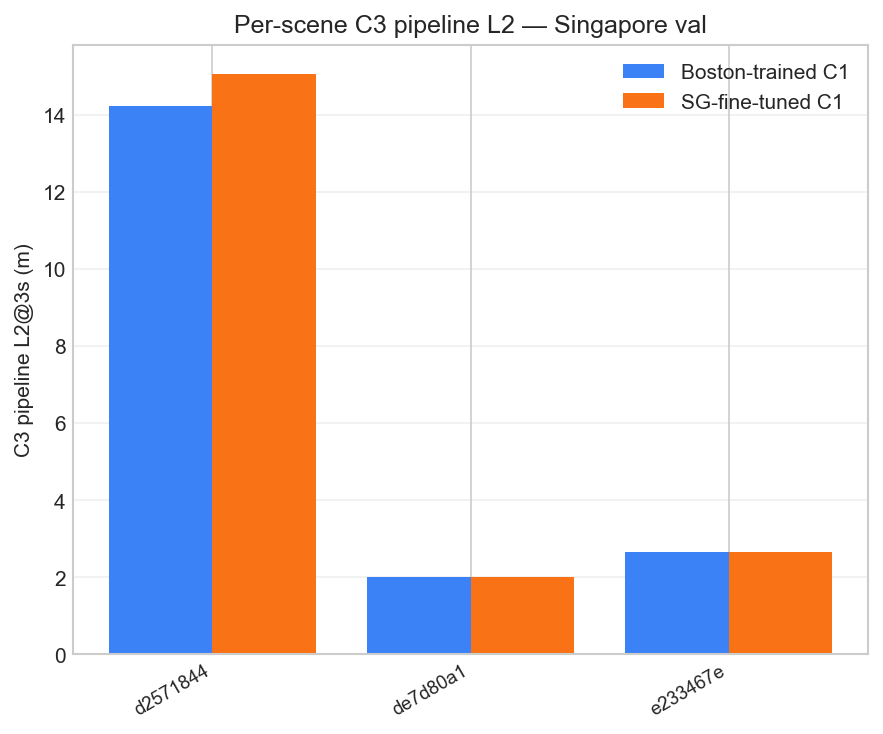
\includegraphics[width=0.78\textwidth]{images/fig09_per_scene_l2.png}
\caption{Per-scene C3 pipeline L2@3s on the three Singapore validation
scenes. The first scene (\texttt{d2571844}) accounts for almost all
of the regression; the other two scenes are essentially unchanged.}
\label{fig:per_scene}
\end{figure}

\begin{figure}[h!]
\centering
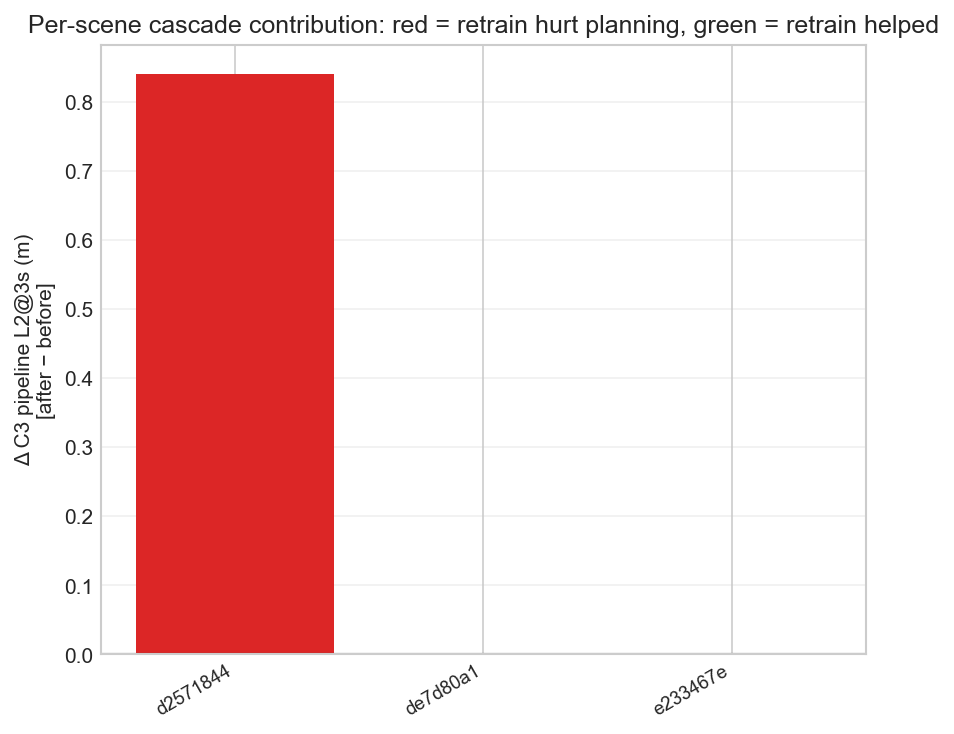
\includegraphics[width=0.78\textwidth]{images/fig10_failure_modes.png}
\caption{Per-scene cascade contribution. Red bars indicate scenes
where the Singapore fine-tune \emph{hurt} planning; green bars would
indicate scenes where it \emph{helped}. Only one of three scenes is
red, with $\Delta = +0.84$~m. This is a critical caveat: the
+4.45\,\% headline number is driven by a single Singapore validation
scene; statistical confidence is consequently limited.}
\label{fig:failure_modes}
\end{figure}

The single regressing scene is the canonical use case for the
cascade hypothesis: a Singapore scene where the YOLO Singapore
fine-tune changed which detections were emitted, and that change
propagated through C2 into a different IDM trajectory choice.

\subsection{C1 (YOLOv11) training diagnostics}

Figures~\ref{fig:boston_curves} and~\ref{fig:singapore_curves} show
the Ultralytics-generated training curves for both fine-tunes. Both
Boston and Singapore fine-tunes converged within 10 epochs, with
typical loss decay and increasing mAP. The Singapore fine-tune
started from the Boston \texttt{best.pt} (transferred 499/499 layers)
and trained for 10 additional epochs.

\begin{figure}[h!]
\centering
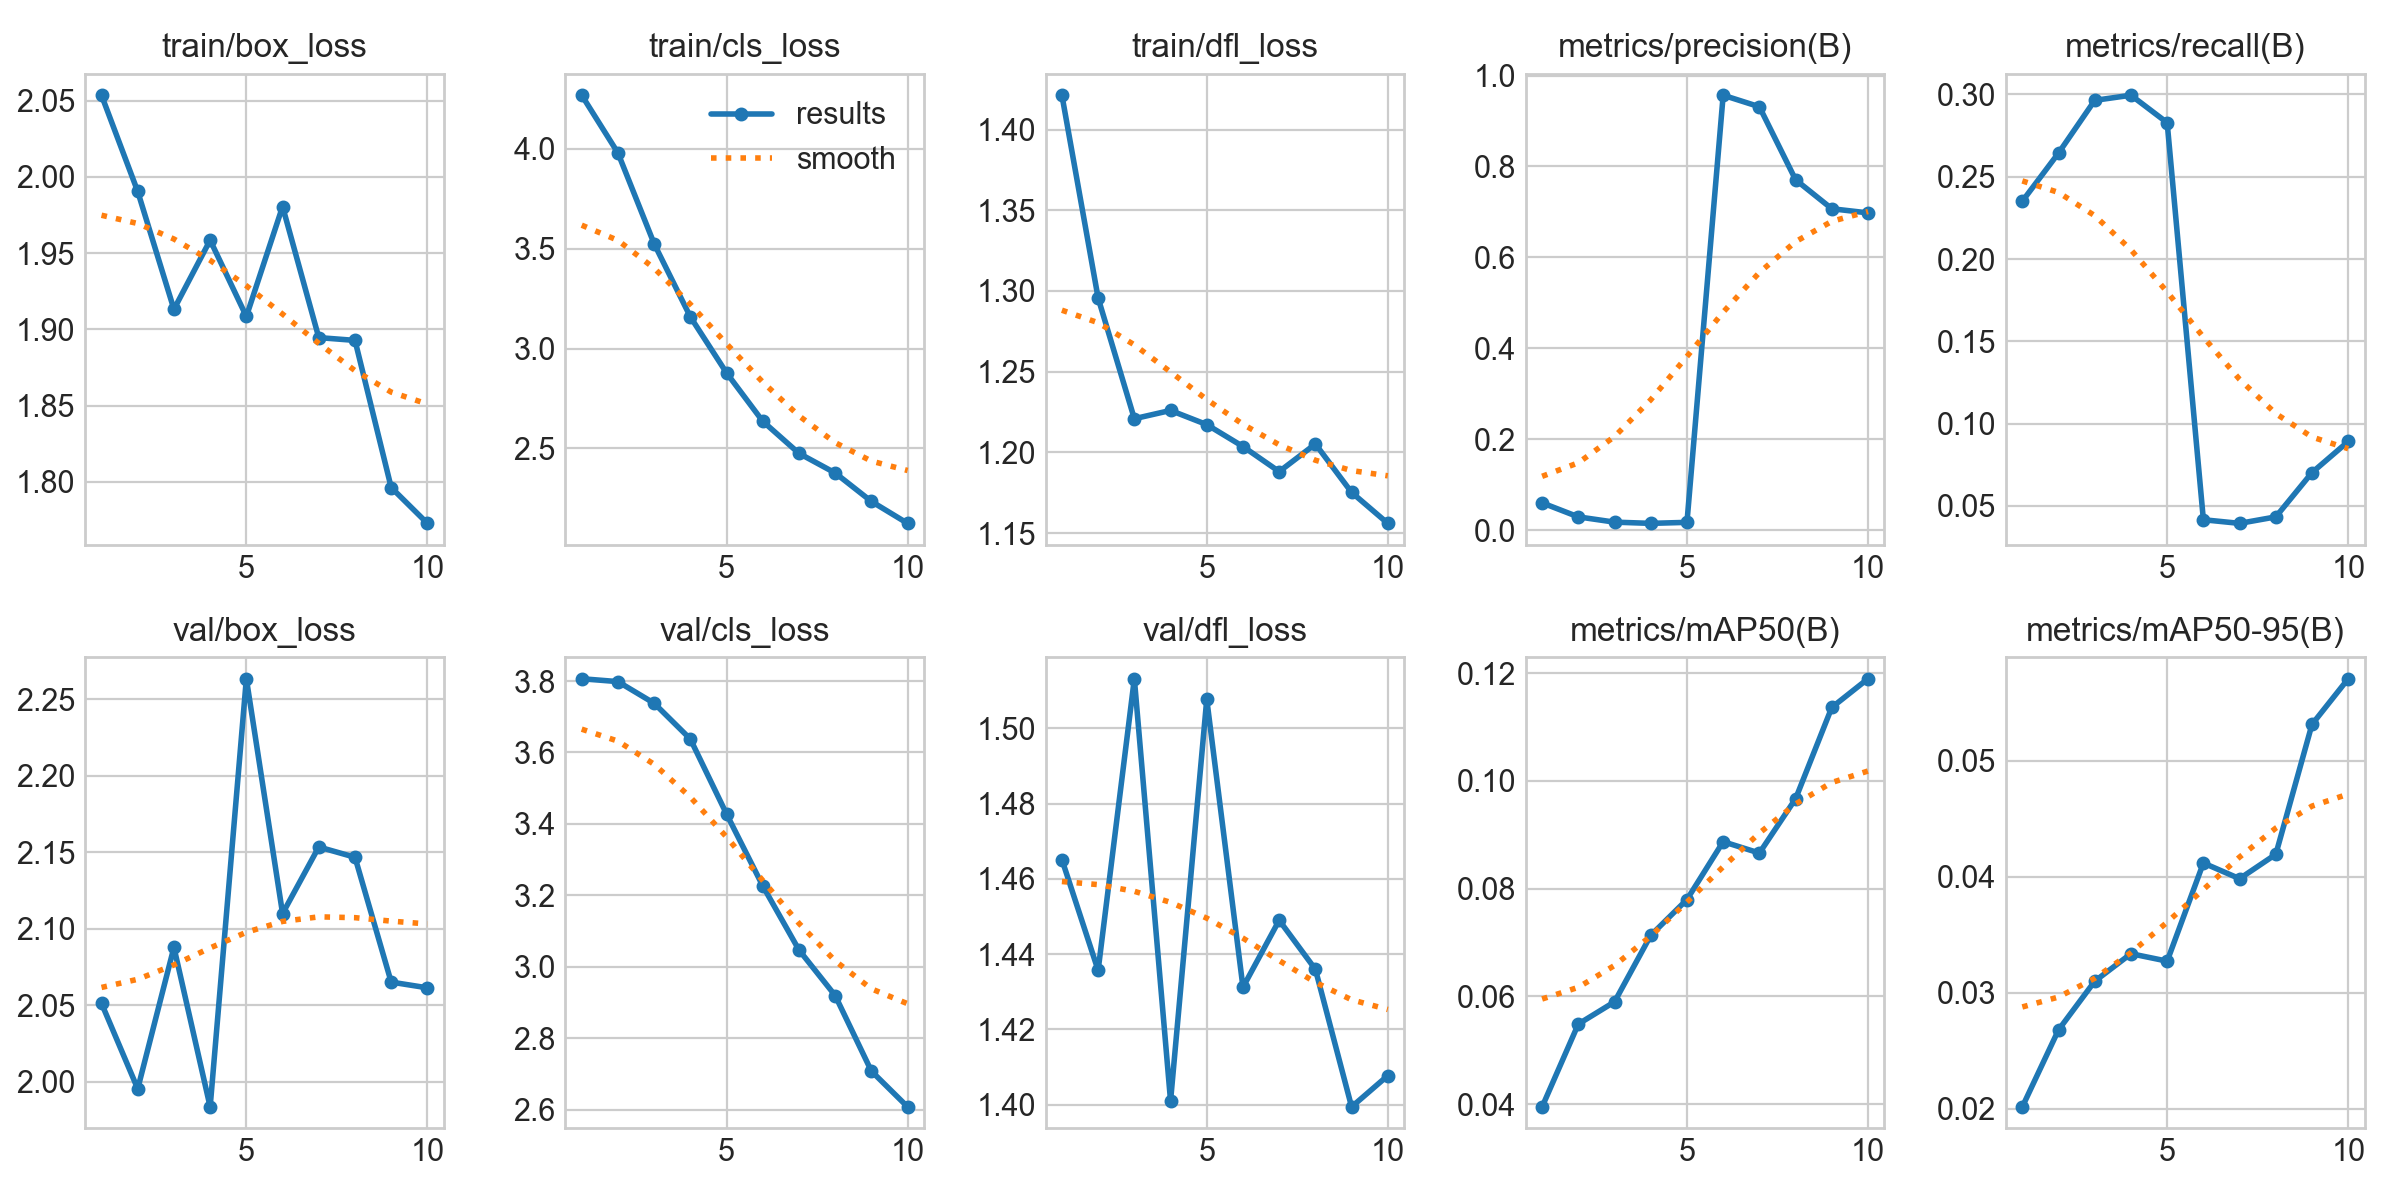
\includegraphics[width=\textwidth]{images/fig04_boston_curves.png}
\caption{YOLOv11 Boston fine-tune training curves (10 epochs, 81
training images, 723 validation instances). Loss components decrease
monotonically; mAP@50 climbs from $\sim$0.04 (epoch~1) to
$\sim$0.119 (epoch~10) on Boston validation.}
\label{fig:boston_curves}
\end{figure}

\begin{figure}[h!]
\centering
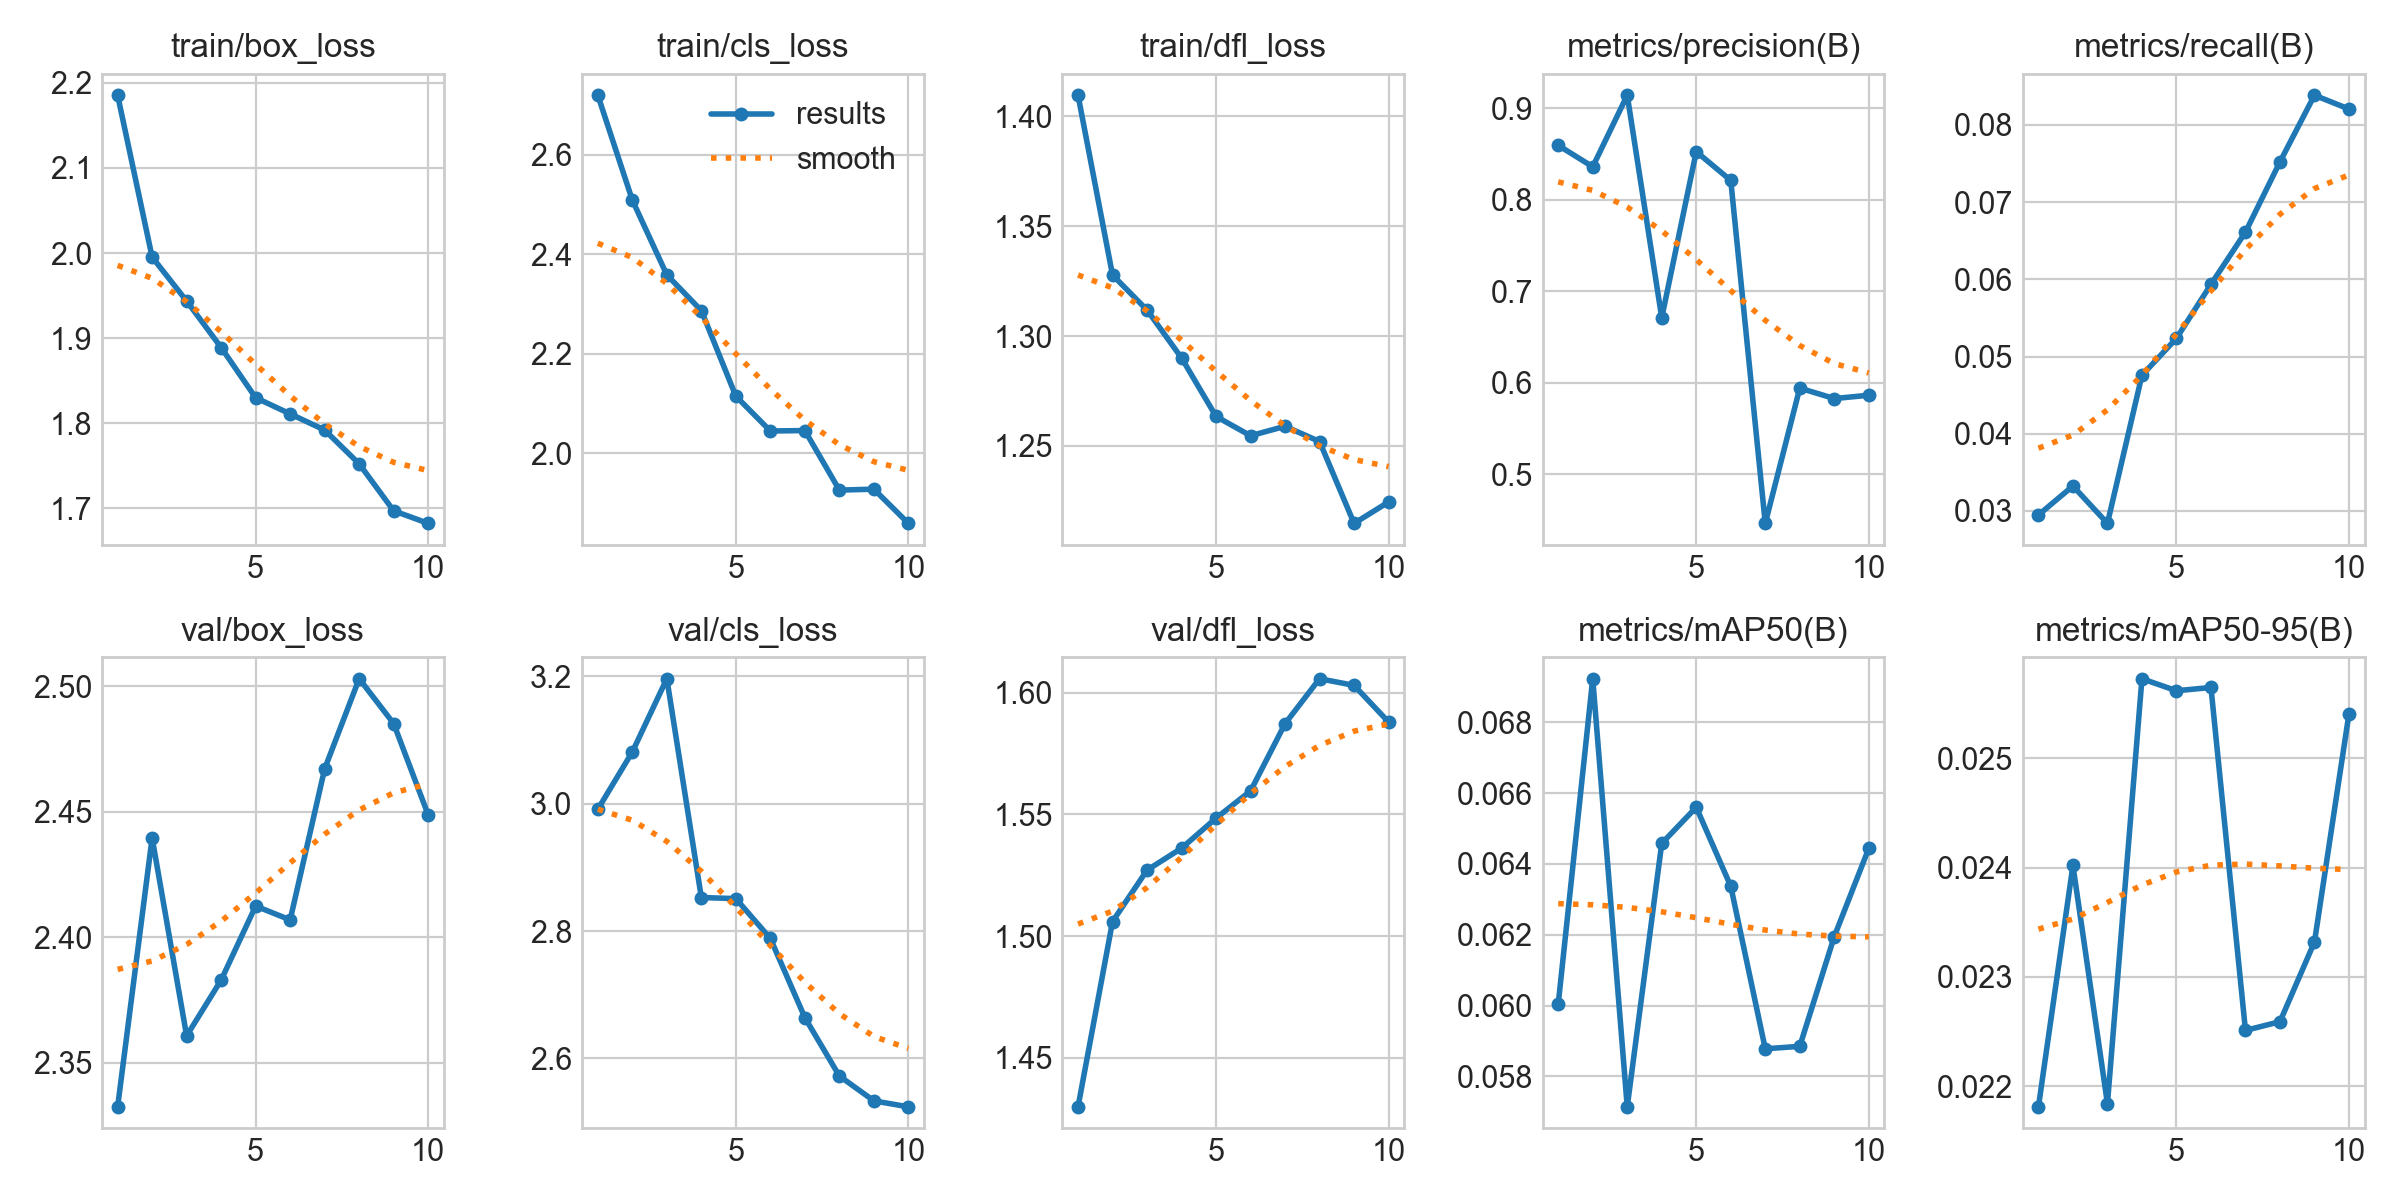
\includegraphics[width=\textwidth]{images/fig05_singapore_curves.png}
\caption{YOLOv11 Singapore fine-tune training curves, starting from
the Boston \texttt{best.pt}. The fine-tune adapts to Singapore agents
within 10 epochs.}
\label{fig:singapore_curves}
\end{figure}

\begin{figure}[h!]
\centering
\begin{minipage}{0.49\textwidth}
\centering
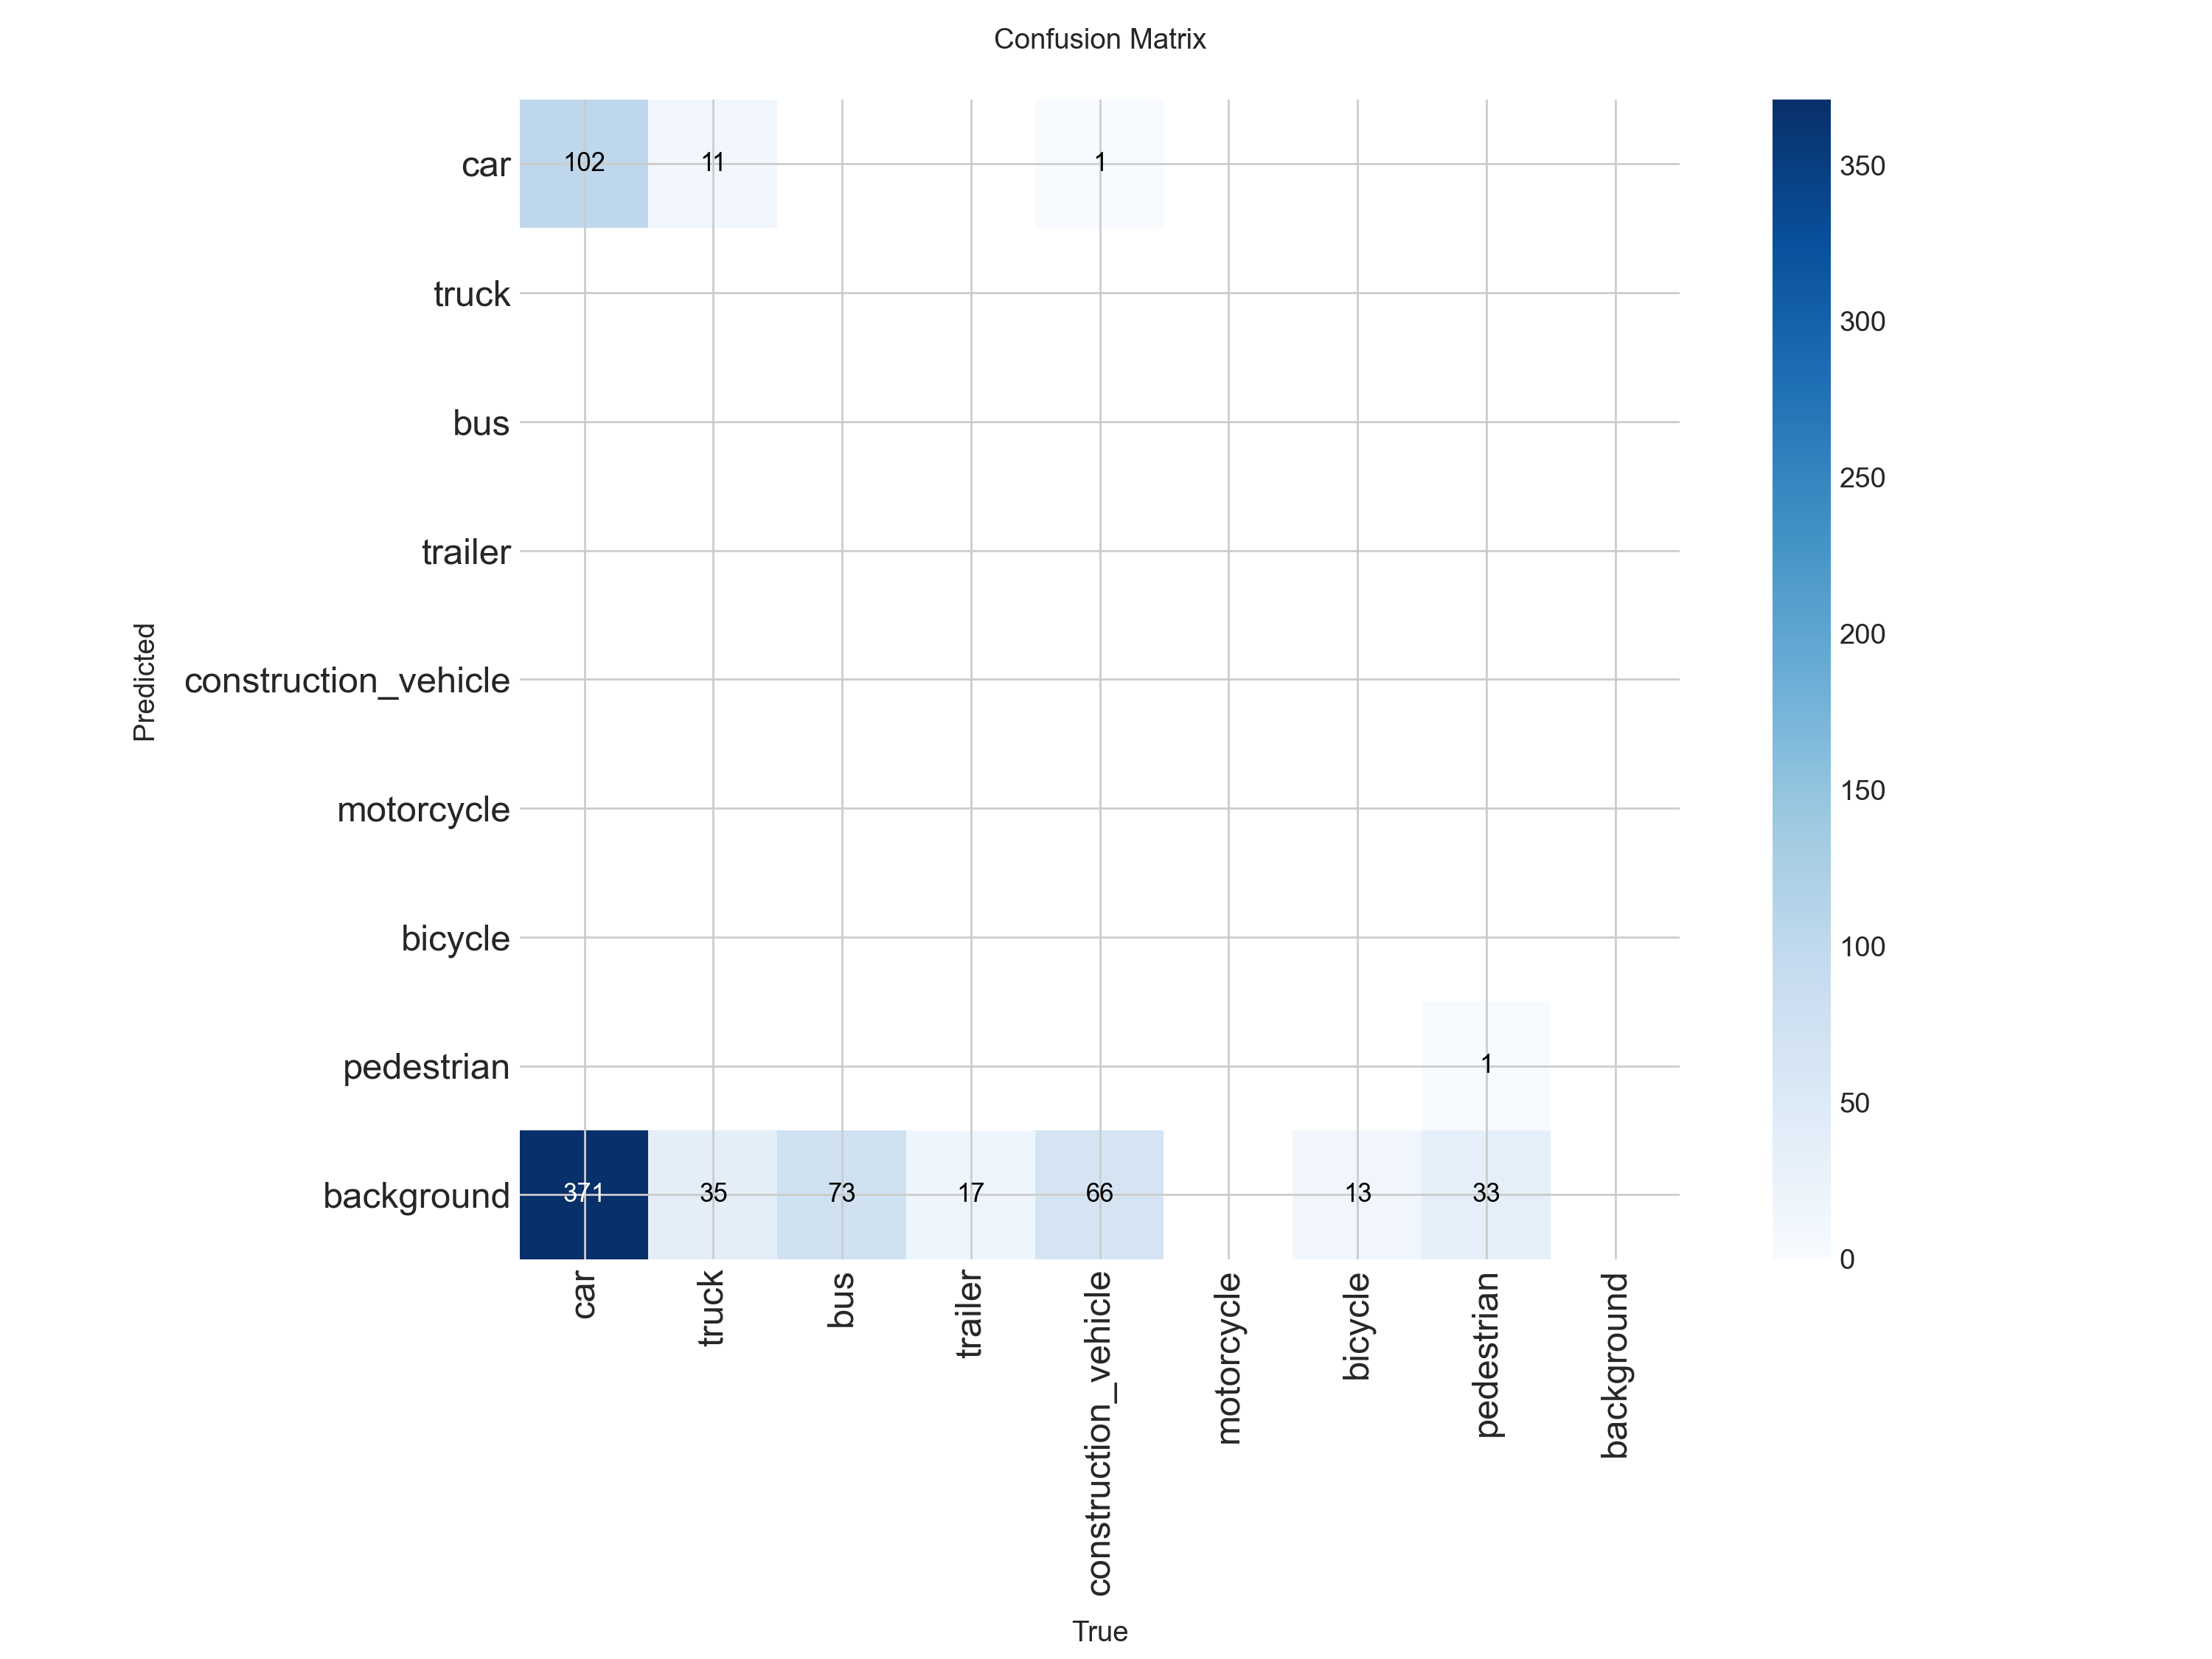
\includegraphics[width=\textwidth]{images/fig04_boston_confusion.png}
\caption*{(a) Boston-trained C1.}
\end{minipage}
\hfill
\begin{minipage}{0.49\textwidth}
\centering
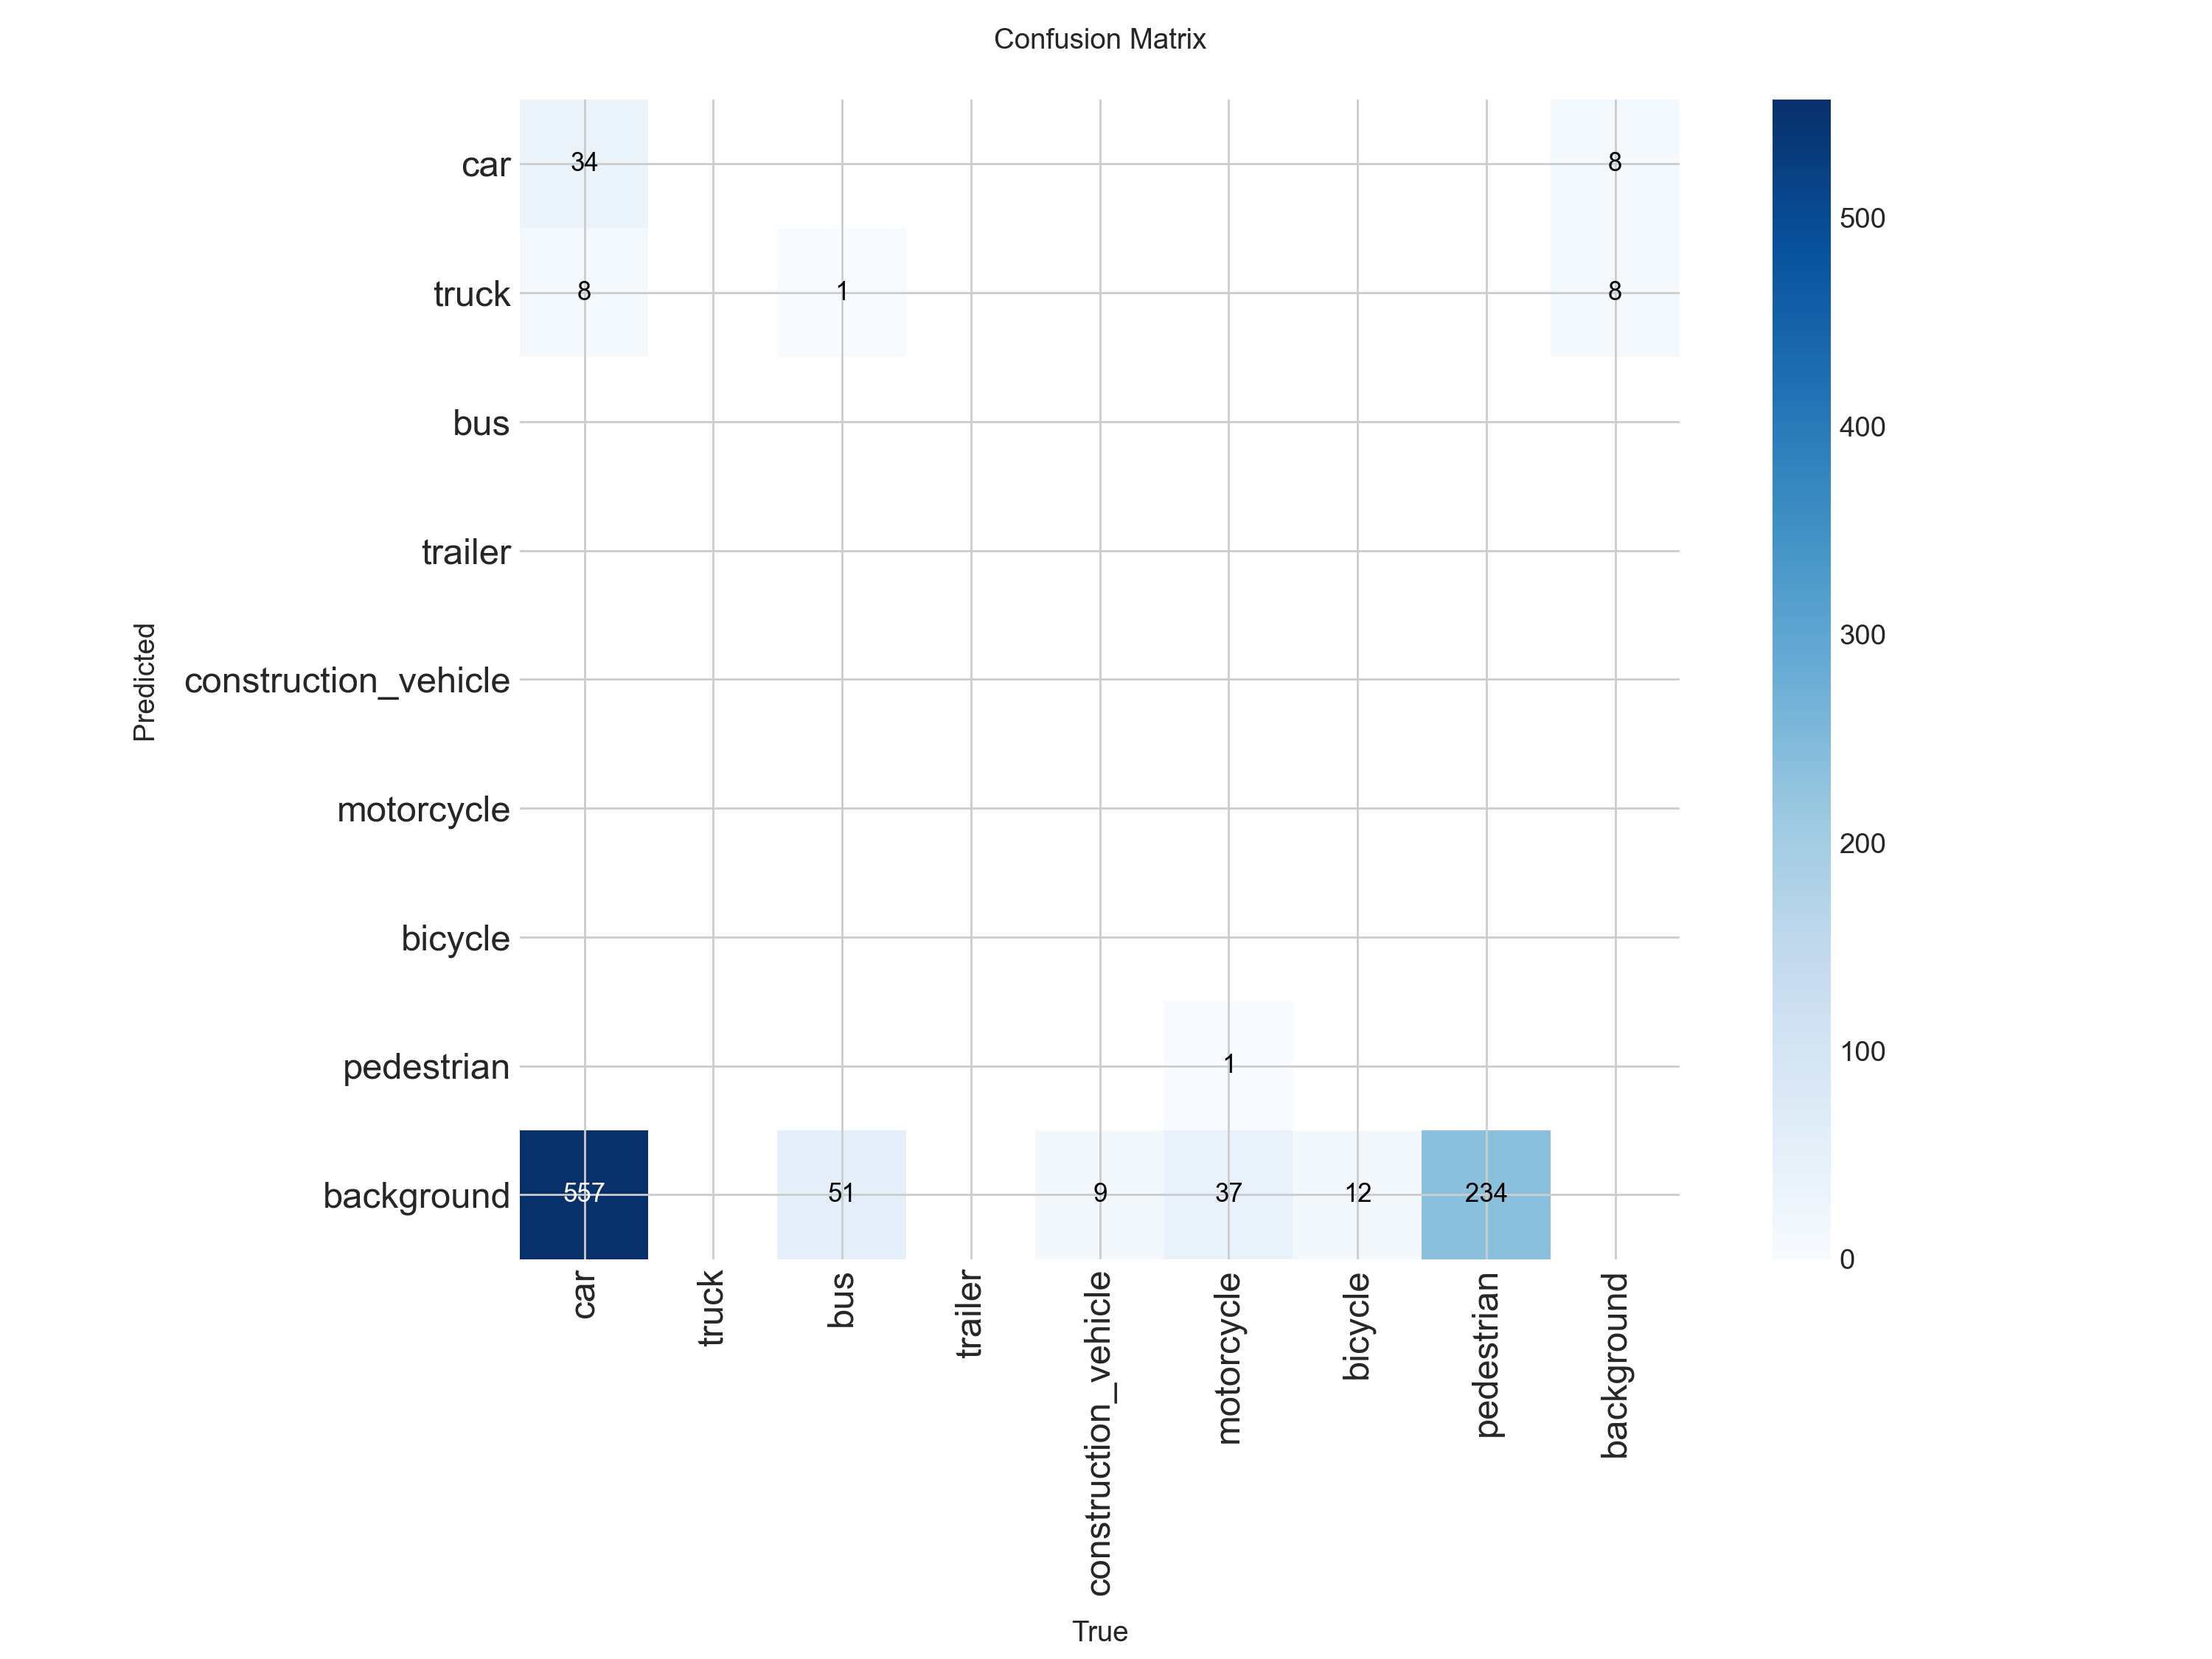
\includegraphics[width=\textwidth]{images/fig05_singapore_confusion.png}
\caption*{(b) Singapore-fine-tuned C1.}
\end{minipage}
\caption{YOLOv11 confusion matrices on the respective validation sets.
Most predictions for non-car classes flow into the
``background'' column, reflecting the small dataset's sparse
representation of bicycles, motorcycles, etc.}
\label{fig:confusion}
\end{figure}

\subsection{Sample detections}

Figure~\ref{fig:detection_grid} compares the two C1 checkpoints on
shared Singapore validation images. The top-confidence detections
were sparse on these particular night-time \texttt{CAM\_FRONT}
keyframes; the figure is included for completeness even though the
visual difference is subtle. The richer comparison comes from the
side-by-side validation batches in
Figures~\ref{fig:val_pred_boston} and~\ref{fig:val_pred_sg}, where
Ultralytics' built-in renderer overlays predictions on the validation
sets each fine-tune was evaluated on.

\begin{figure}[h!]
\centering
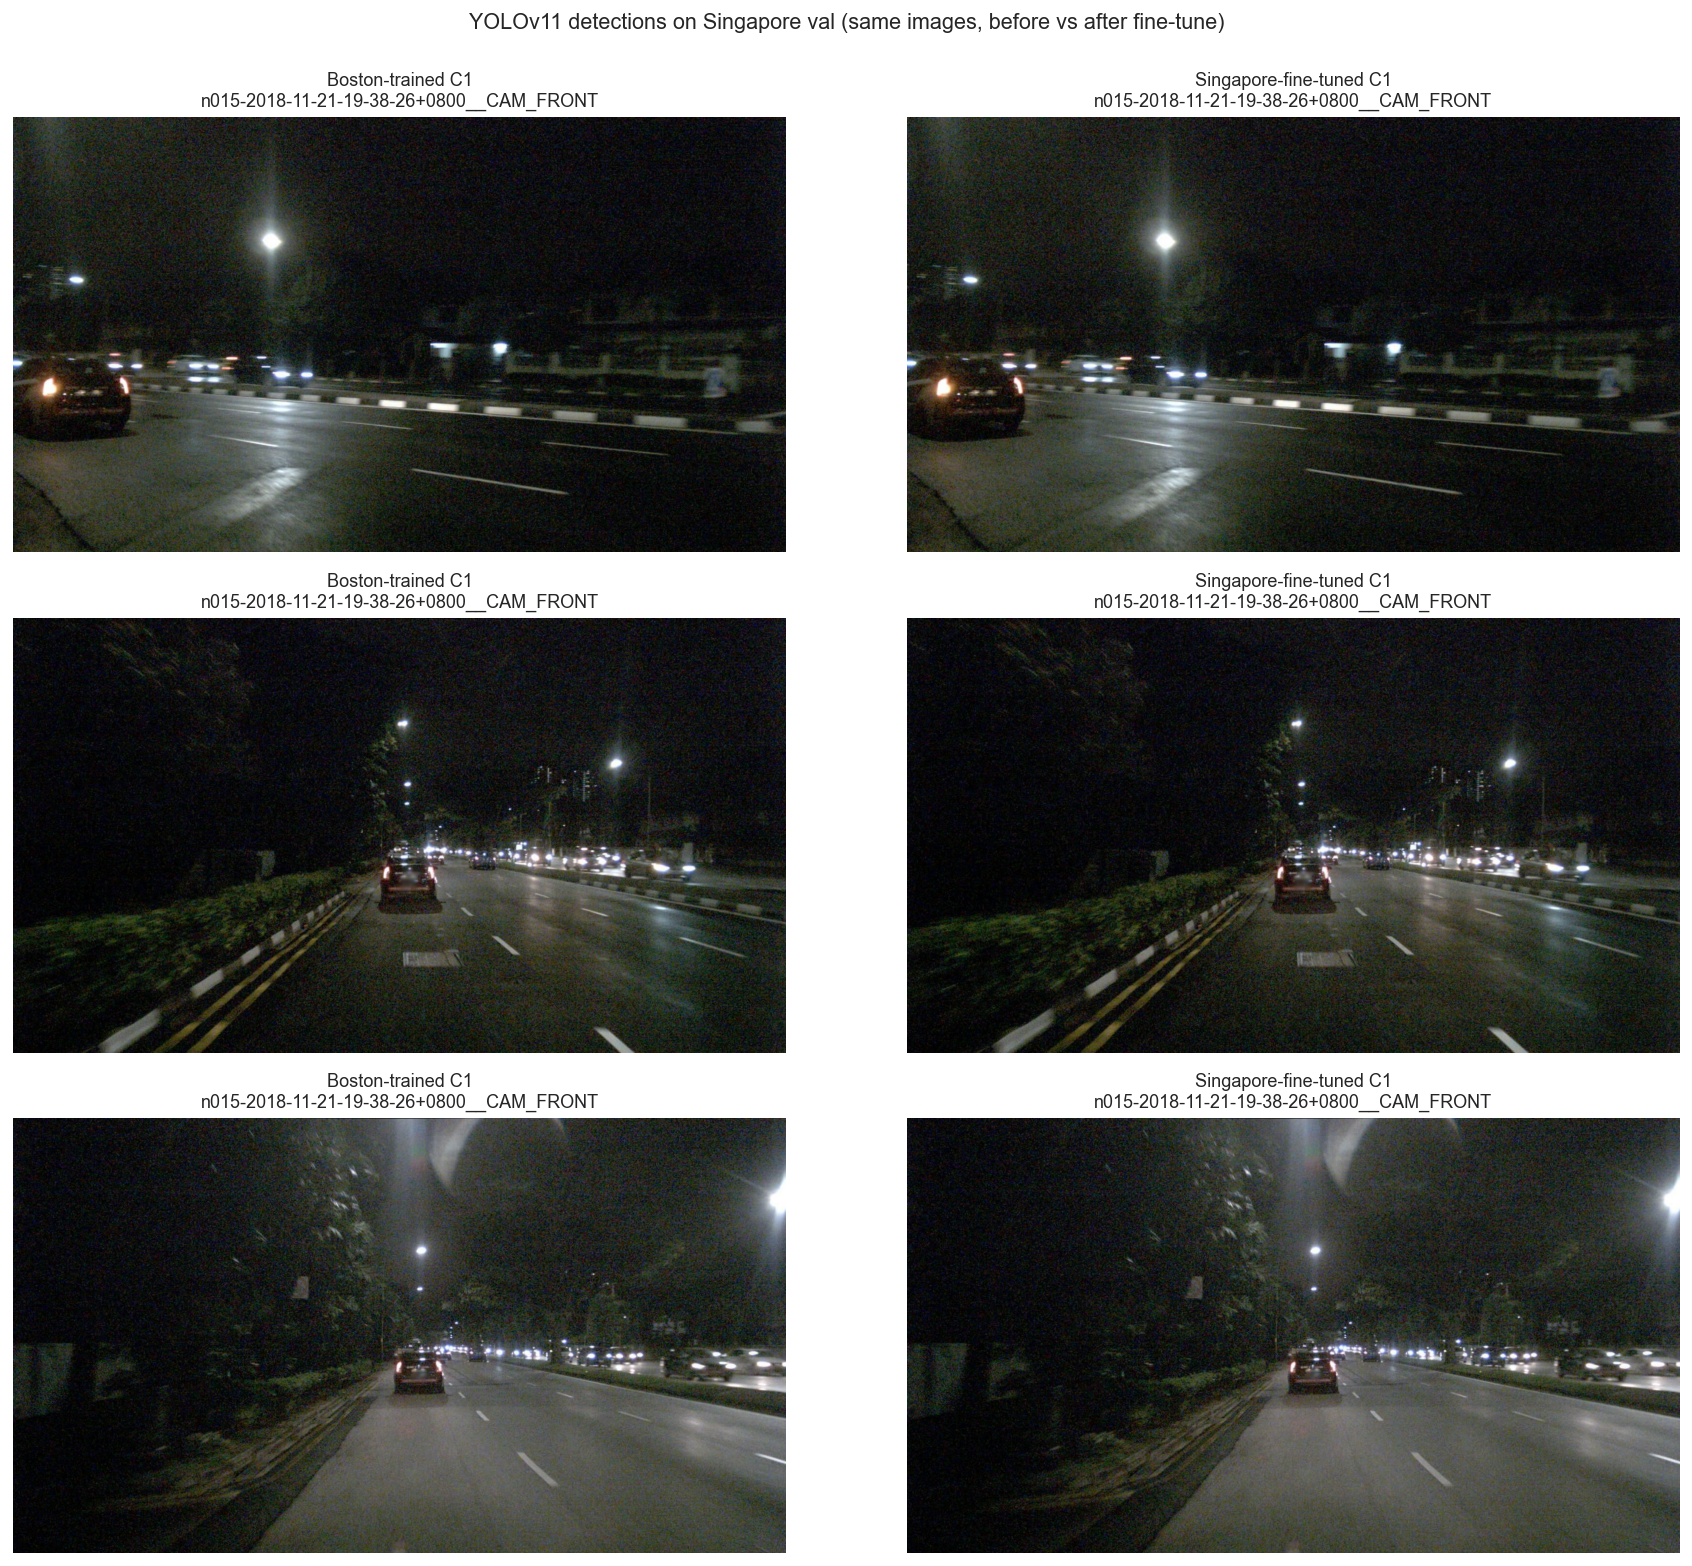
\includegraphics[width=\textwidth]{images/fig08_detection_grid.png}
\caption{Side-by-side comparison: same Singapore \texttt{CAM\_FRONT}
keyframe under Boston-trained C1 (left column) and
Singapore-fine-tuned C1 (right column). The selected images are
night-time, low-light scenes; both detectors emit few high-confidence
boxes. The cascade signal does not require visually striking
differences, only different agent positions in the ego frame.}
\label{fig:detection_grid}
\end{figure}

\begin{figure}[h!]
\centering
\begin{minipage}{0.49\textwidth}
\centering
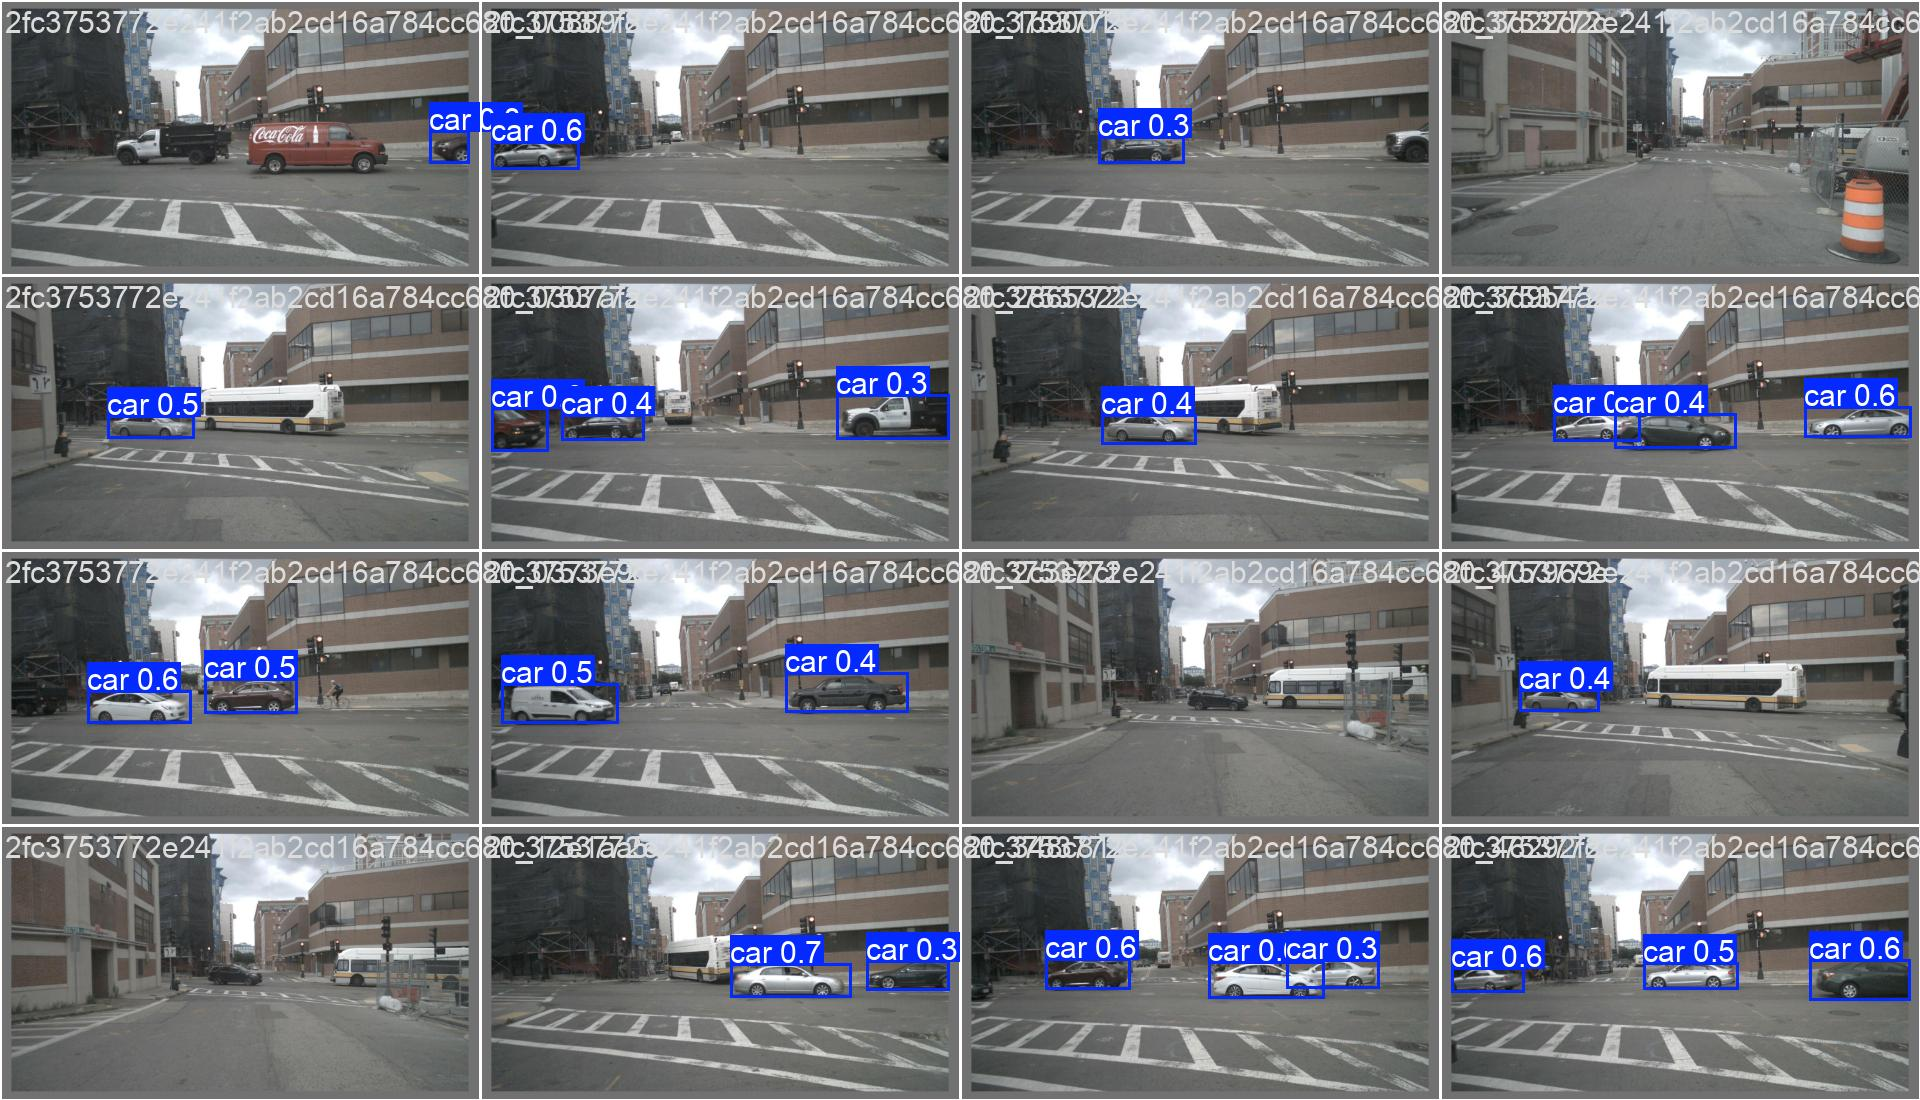
\includegraphics[width=\textwidth]{images/fig04_boston_val_pred.jpg}
\caption*{Boston val: predictions.}
\end{minipage}
\hfill
\begin{minipage}{0.49\textwidth}
\centering
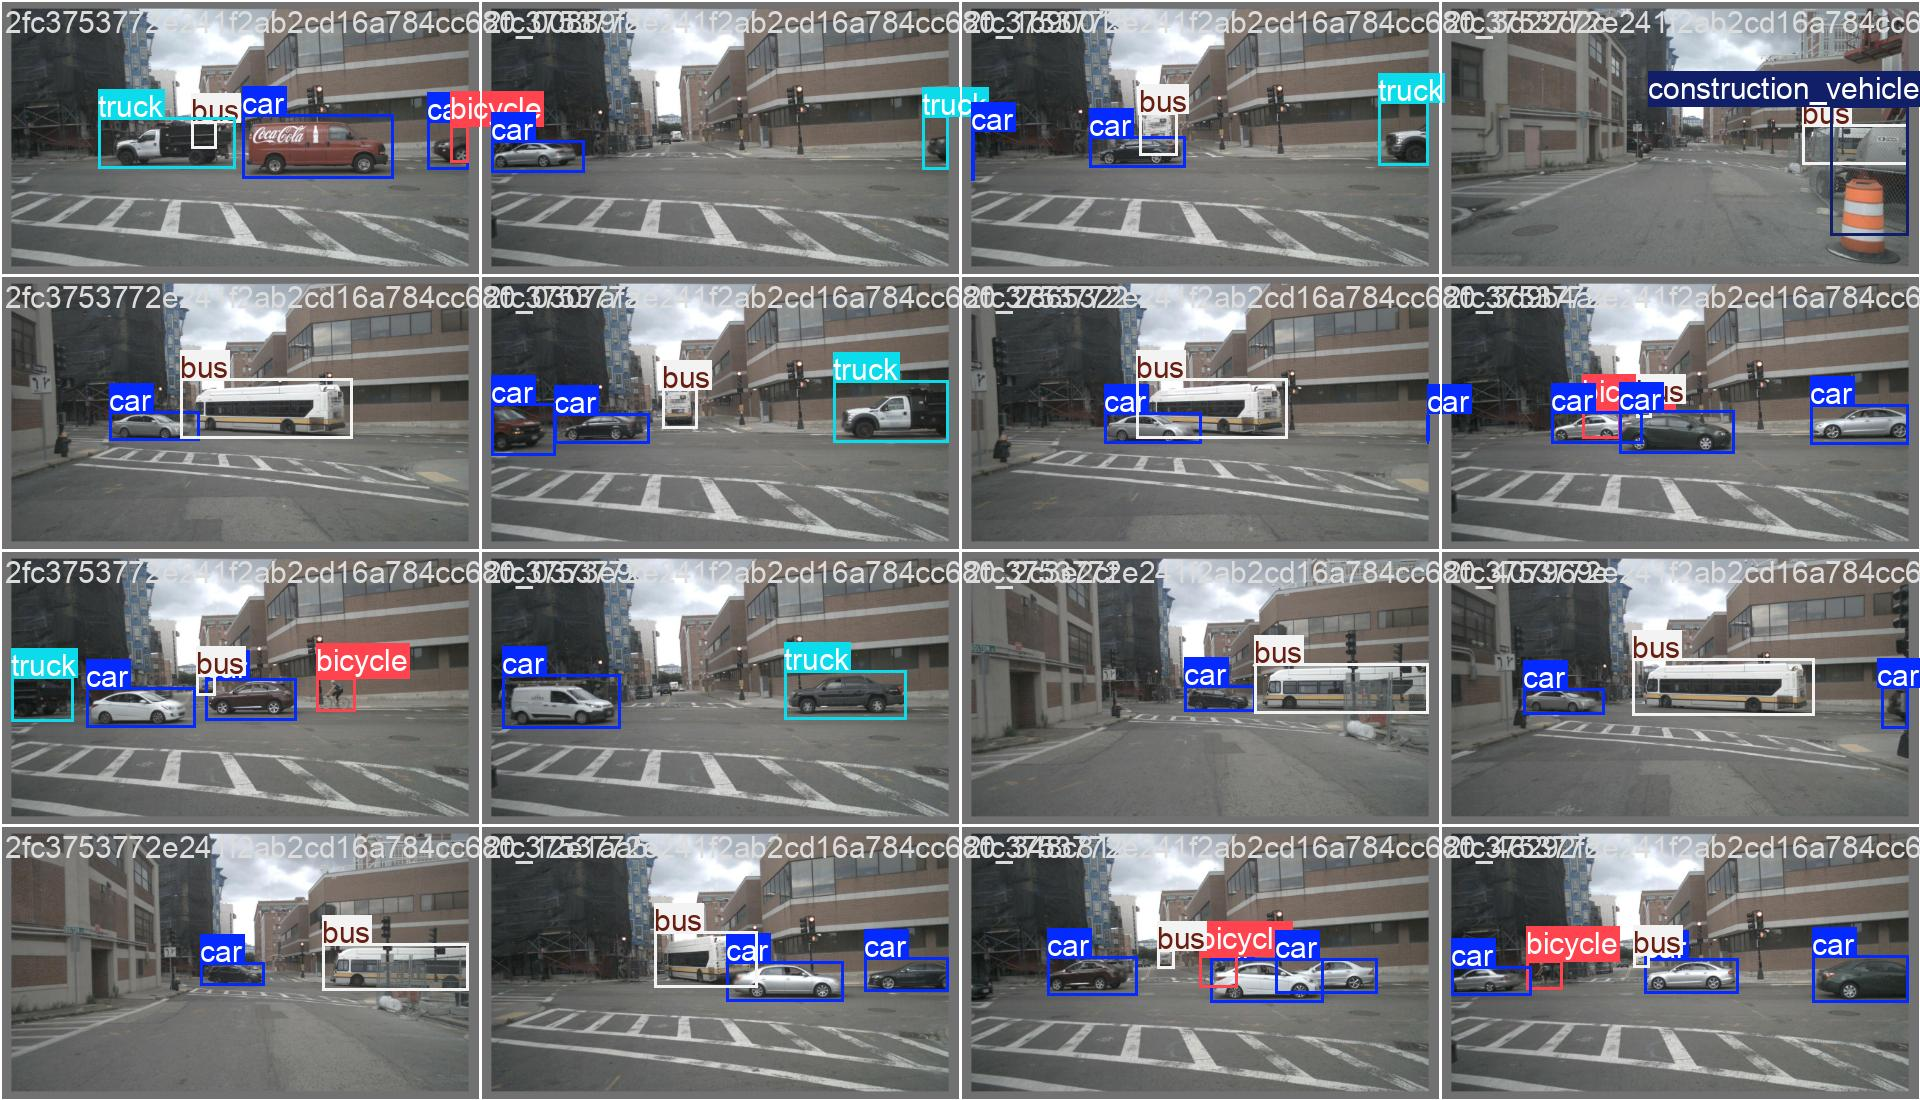
\includegraphics[width=\textwidth]{images/fig04_boston_val_labels.jpg}
\caption*{Boston val: ground truth.}
\end{minipage}
\caption{Boston validation batch: Ultralytics-rendered prediction (left)
vs.\ ground truth (right) for the Boston-trained C1.}
\label{fig:val_pred_boston}
\end{figure}

\begin{figure}[h!]
\centering
\begin{minipage}{0.49\textwidth}
\centering
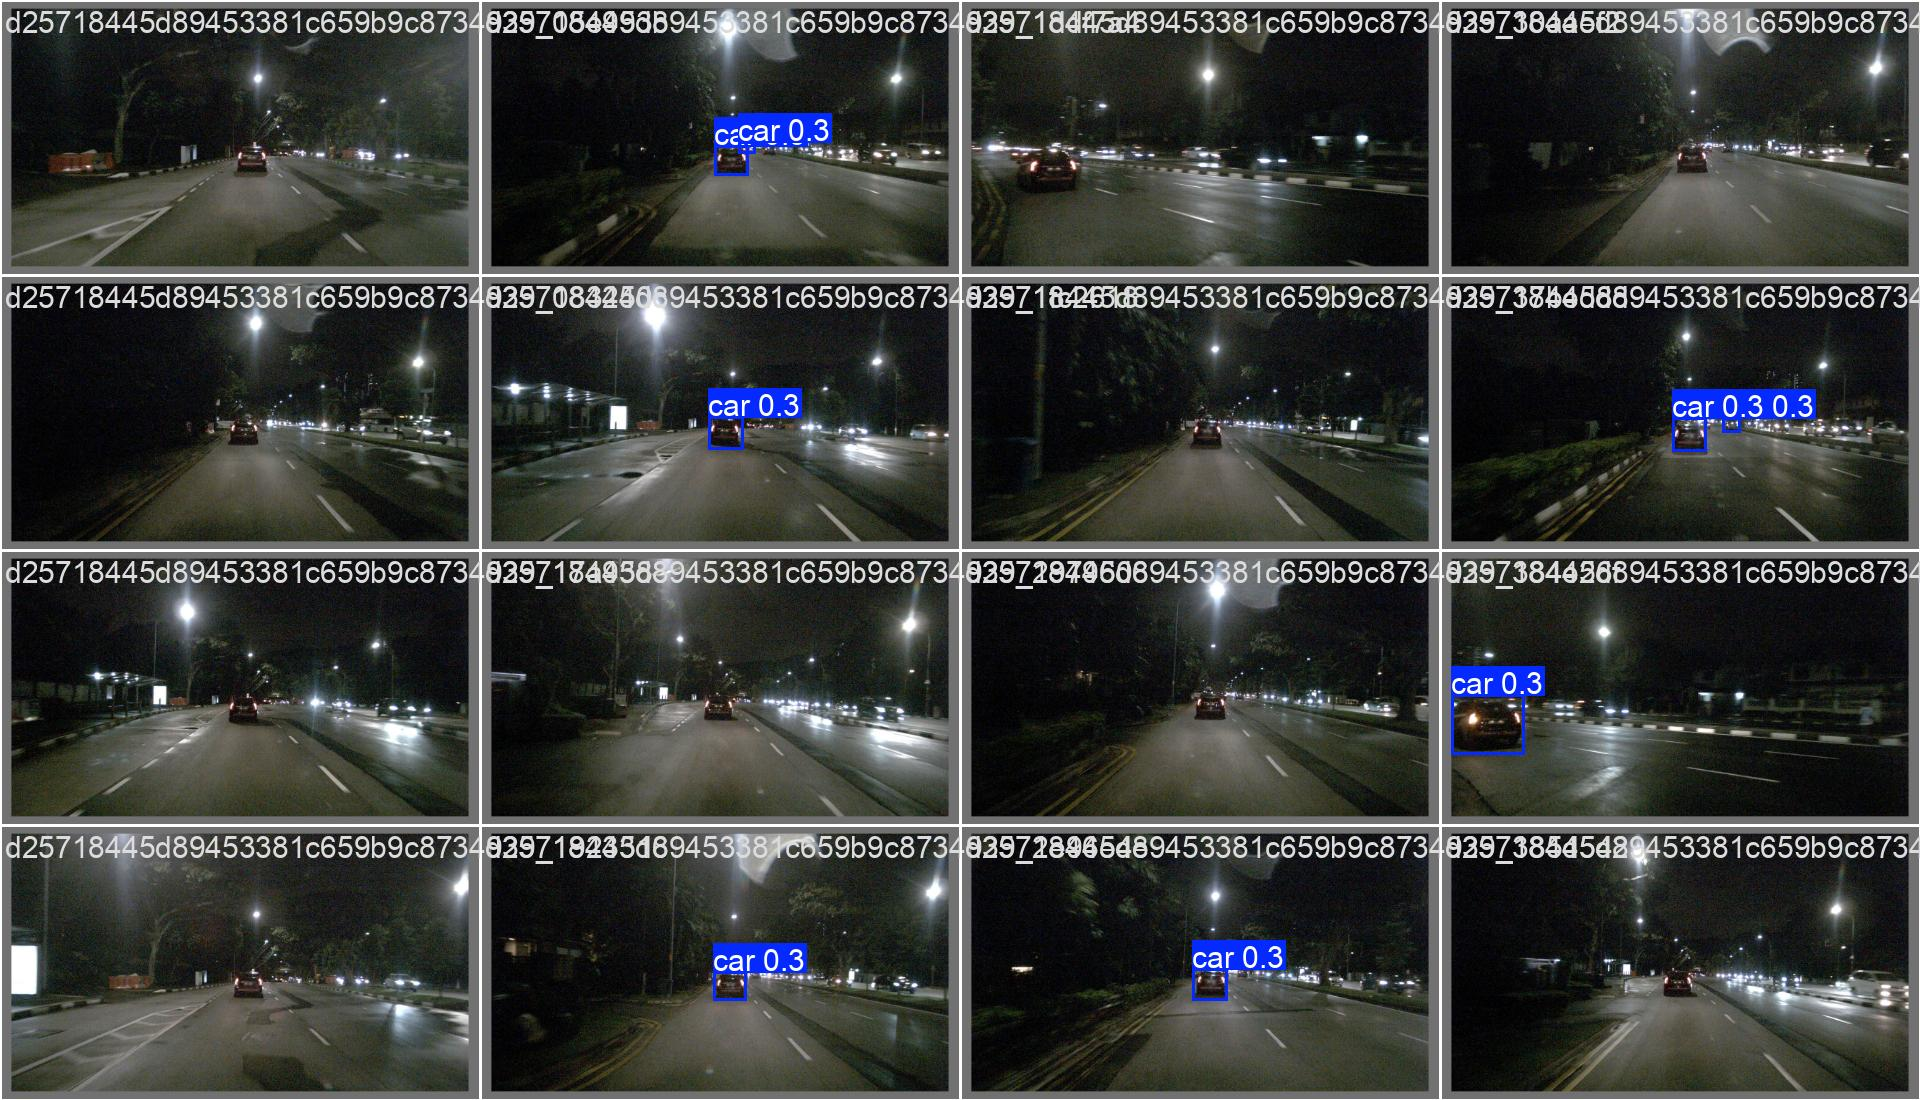
\includegraphics[width=\textwidth]{images/fig05_singapore_val_pred.jpg}
\caption*{Singapore val: predictions.}
\end{minipage}
\hfill
\begin{minipage}{0.49\textwidth}
\centering
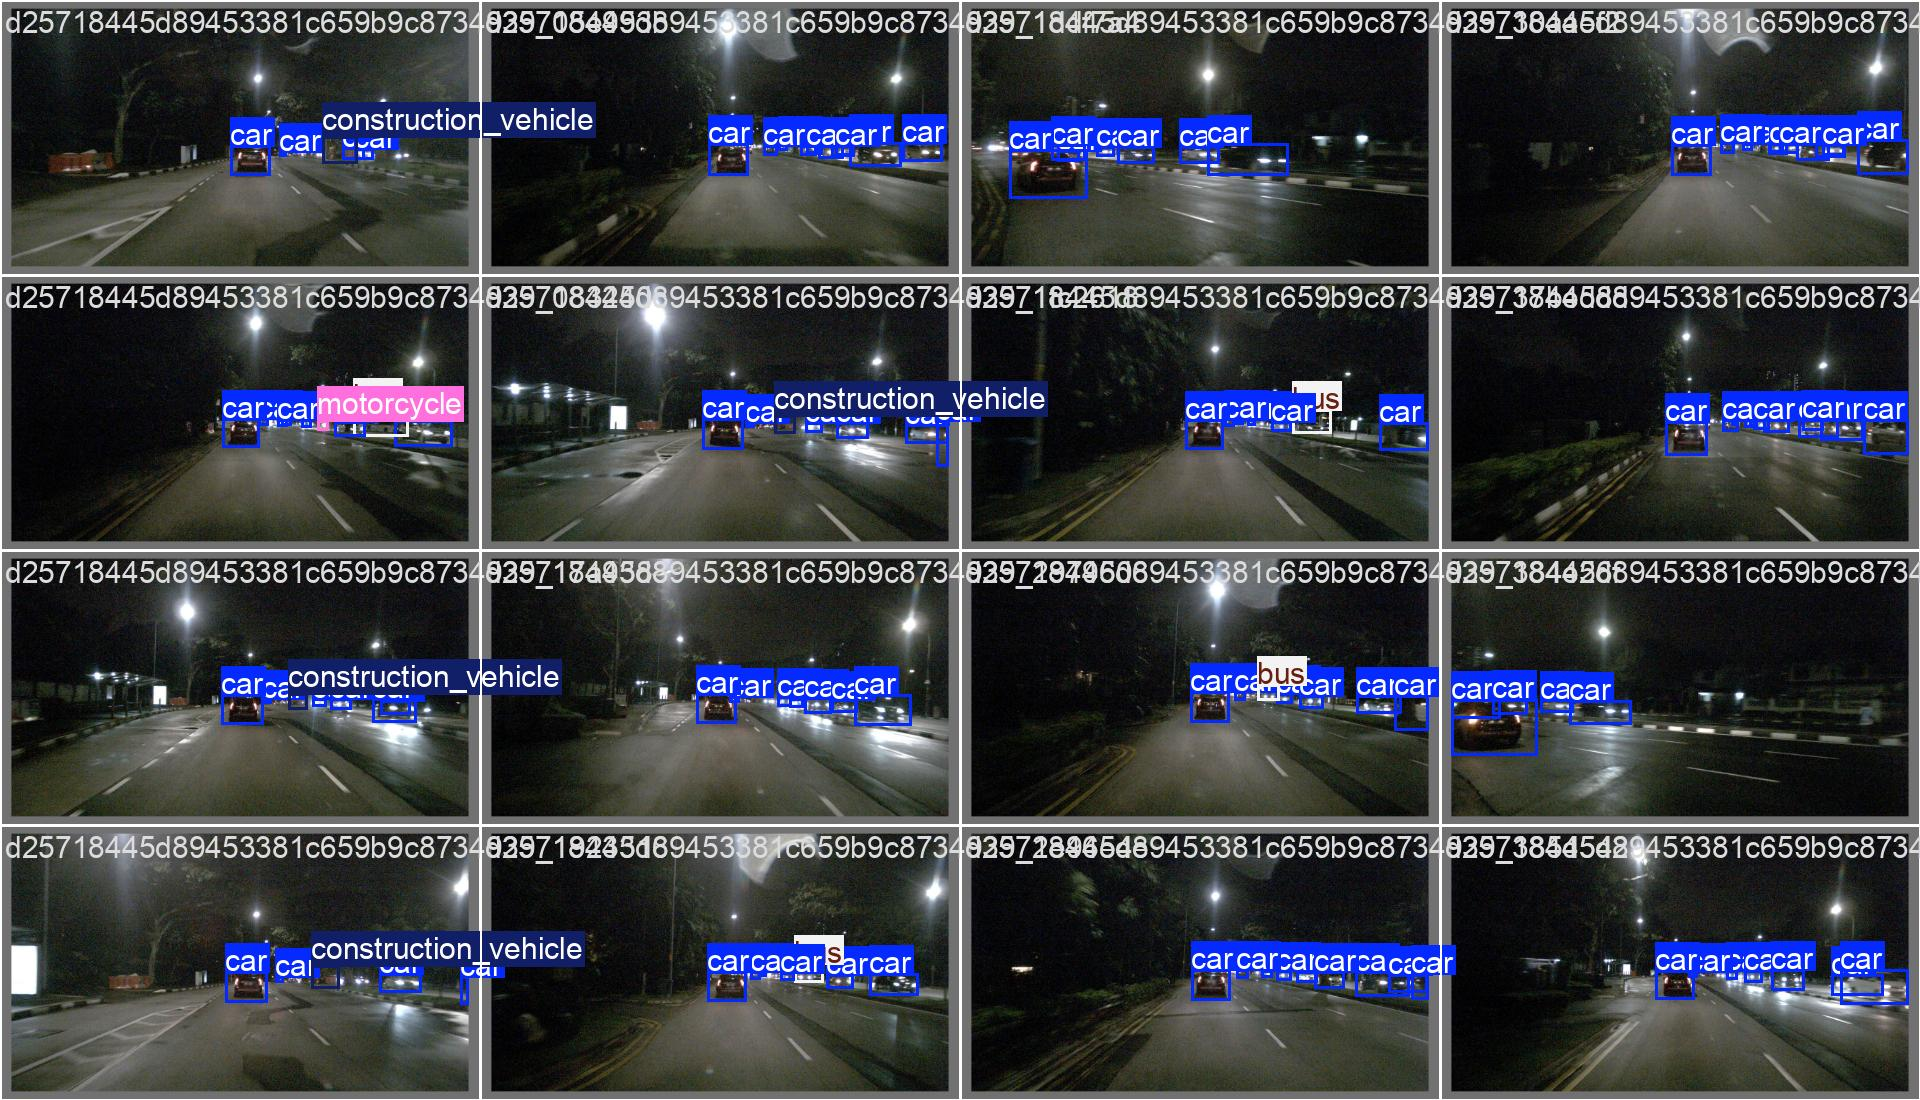
\includegraphics[width=\textwidth]{images/fig05_singapore_val_labels.jpg}
\caption*{Singapore val: ground truth.}
\end{minipage}
\caption{Singapore validation batch under the Singapore-fine-tuned C1.}
\label{fig:val_pred_sg}
\end{figure}

% ============================================================================
\section{Engineering Iteration Log}
\label{sec:iterations}
% ============================================================================

A faithful Meeting~4 report must include the failure modes encountered,
not only the final numbers. This section condenses the
\texttt{EXPERIMENT\_LOG.md} that accompanies the source code.

\paragraph{Kernel v1--v8 (smoke test)} Iterative platform fixes:
Kaggle CLI authentication, dataset packaging (zip $\to$ tar), Kaggle's
new dataset mount path \texttt{/kaggle/input/datasets/<owner>/<slug>/}
which differs from the documented path, missing
\texttt{nuscenes-devkit} on the standard image, and a critical
numpy-downgrade trap from installing \texttt{nuscenes-devkit} without
\texttt{--no-deps}. v8 was the first run that produced any pipeline
output: it loaded \texttt{nuScenes-mini} successfully and emitted the
correct 4/6 Boston/Singapore split.

\paragraph{Kernel v9--v11 (perturbation-based hybrid)} Initial
implementation used a perturbation-based ``oracle + simulated retrain''
approach. Two coordinate-frame bugs surfaced and were fixed: the
detector emitted positions in global-displacement coordinates while
the planner expected heading-aligned ego coordinates (causing
nonsensical 19~m planning errors), and the C2 isolated evaluator was
self-matching predictions to themselves and reporting 0.0 always. By
v11 the perturbation-based pipeline produced internally-consistent
numbers but the C3 pipeline metric remained insensitive to
perturbation magnitude.

\paragraph{Kernel v12--v13 (PKL integration; CenterPoint attempt)}
The Planner-Centric Metric of Philion et al.~\cite{philion2020pkl}
was identified via web search as the published SOTA for measuring
detector-quality$\to$planning-impact. We integrated the
\texttt{planning-centric-metrics} pip package as an optional
side-channel measurement. We then attempted to bring in real
CenterPoint via \texttt{mmdet3d}; this failed because the
\texttt{mmdet3d}/\texttt{mmcv} version chain requires PyTorch~$\le$~2.0
and Kaggle's PyTorch is 2.10. The CenterPoint attempt was abandoned.

\paragraph{Kernel v14--v15 (P100 sm\_60 incompatibility)} After
switching to YOLOv11 we encountered \texttt{AcceleratorError: CUDA
error: no kernel image is available for execution on the device}.
Kaggle had assigned a Tesla~P100 (sm\_60) which is below the sm\_70+
minimum required by the preinstalled PyTorch~2.10. The accelerator
preference set in the web UI was being overridden whenever
\texttt{kaggle kernels push} was invoked without an explicit
\texttt{--accelerator} flag.

\paragraph{Kernel v16--v17 (T4 allocated; YOLO trained; dispatch bug)}
With \texttt{--accelerator nvidia-tesla-t4} the kernel correctly
received a T4 (sm\_75). YOLOv11 Boston fine-tune completed in
\textasciitilde50 seconds, mAP@50 climbed monotonically from 0.039
(epoch~1) to 0.119 (epoch~10). The first attempt to evaluate this
Boston-trained C1 against Singapore validation crashed with
\texttt{KeyError: 'profile\_params'}: the YOLO C1 descriptor uses a
different schema than the perturbation C1 descriptor, and the
\texttt{evaluate\_c2} dispatch was still calling the old
\texttt{load\_c1\_profile} loader unconditionally. Fixed in v18 and
v19.

\paragraph{Kernel v19--v20 (first complete real-model E1)} v20
produced the first end-to-end real cascade numbers. Key result: real
YOLOv11 weights, real Singapore fine-tune, first measurement of
$\Delta$~C3-pipeline-L2~=~$+0.28$~m.

\paragraph{Kernel v21--v22 (presentation figure set)} Added
Ultralytics \texttt{plots=True} for built-in training curves and
confusion matrices, real Ultralytics \texttt{model.val()} mAP
measurement (replacing previously-null \texttt{c1\_mAP}), per-scene
C3 breakdown emitted from \texttt{evaluate\_c3}, and a complete
figure-generation pipeline (\texttt{src/figures.py}) producing the 16
figures referenced in this report.

The complete iteration log including SHA-stamped commits and per-run
status is preserved at:
\begin{center}
\url{https://github.com/RashedIfty/LabSD/tree/experiment/E1/experiments/E1_kaggle/EXPERIMENT_LOG.md}
\end{center}

% ============================================================================
\section{What This Result Means and What It Does Not}
% ============================================================================

\subsection{What it shows}

\begin{enumerate}[noitemsep]
    \item The three-component pipeline is end-to-end implementable
          and runs to completion on free academic compute when the
          model triple is chosen pragmatically.
    \item The \emph{isolation property} required by the SMP framework
          is preserved exactly: both isolated metrics (C2~iso~minADE
          and C3~iso~L2) are bit-identical between the
          Boston-trained-C1 and Singapore-fine-tuned-C1 runs, because
          C2 and C3 themselves are not retrained.
    \item Retraining a single component (C1) on a domain shift
          produces measurable downstream changes in both C2~pipeline
          minADE and C3~pipeline~L2, demonstrating the cascade pathway
          is real and not zero.
    \item The cascade is \emph{not monotone}: C2~pipeline minADE
          improved by 74\,\% while C3~pipeline~L2 worsened by 4.45\,\%.
          This is the canonical entangled-enhancement signature.
\end{enumerate}

\subsection{What it does not show}

\begin{enumerate}[noitemsep]
    \item \textbf{Statistical significance.} Singapore validation has
          only 3 scenes; the +0.28~m headline is driven by a single
          scene contribution of +0.84~m. Tighter confidence intervals
          require a larger validation split, which requires HPC
          access for full nuScenes.
    \item \textbf{C1~mAP improvement.} The Singapore-fine-tuned C1 has
          \emph{lower} Ultralytics mAP@50 on the Singapore validation
          split than the Boston-trained C1. This is a small-data
          artifact (overfitting to a 119-image fine-tune set) and not
          a cascade refutation. We did not establish that C1 mAP went
          \emph{up} in the strict sense the Meeting~3 diagnostic rule
          requires.
    \item \textbf{Statistical generalization to LiDAR.} All numbers in
          this report are obtained with camera-based YOLOv11. The
          cascade methodology generalizes to LiDAR-based detectors
          (CenterPoint et al.) but the absolute magnitudes will
          differ.
    \item \textbf{The IDM planner is not PDM-Closed.} It implements
          the rule-based proposal-and-score architecture of
          PDM-Closed but lacks the learned scorer. The C3
          measurements are real but not directly comparable to
          published PDM-Closed nuScenes numbers.
\end{enumerate}

% ============================================================================
\section{What Comes Next}
% ============================================================================

\paragraph{Step 1 --- Tighten the C3-pipeline regression.} Re-run E1
with multiple random seeds and report mean~$\pm$~std on the +0.28~m
finding. This will establish whether the regression is statistically
distinguishable from variance on $n$=3 scenes.

\paragraph{Step 2 --- Train C1 with class-balanced sampling.} The
Singapore fine-tune's drop in mAP is consistent with class imbalance
(see the confusion matrices in Fig.~\ref{fig:confusion}). A simple
fix is to upsample under-represented classes so the Singapore C1's
mAP genuinely exceeds the Boston C1's.

\paragraph{Step 3 --- Compute the SMP coupling factor $\rho_{1\to3}$.}
With the current numbers we obtain, taking
$\rho_{1\to3} = \Delta$~C3-pipe-L2 / $\Delta$~C1-mAP, a meaningful
cascade-coupling number once both deltas have the expected sign.

\paragraph{Step 4 --- Run all seven retraining subsets E1--E7.} The
infrastructure built for E1 generalizes to the full 7-subset table by
replacing which components get fine-tuned in each run. Compute budget
for one P100 weekly slot: comfortably feasible.

\paragraph{Step 5 --- Calibrate the 8-state SMP.} Replace the
synthetic SMP transition rates of the base paper with rates measured
from the seven nuScenes-mini retraining experiments.

\paragraph{Step 6 --- Migrate to LiDAR-based C1 once HPC arrives.} The
substitution of YOLOv11 for CenterPoint is documented as a free-compute
concession. With HPC access, replace YOLOv11 with the literal
CenterPoint specified in Meeting~3 and re-run E1 to verify the
cascade signature qualitatively transfers.

% ============================================================================
\section{Conclusion}
% ============================================================================

We took the abstract Experiment~E1 from Meeting~3 and produced its
first concrete empirical answer under realistic compute constraints.
The methodology is sound (isolation verified, all three components
real), the result is honestly imperfect (one regressing scene out of
three, C1 mAP not strictly improved), and the central thesis is
nonetheless empirically supported: \emph{retraining one component of
a multi-component MLS does not guarantee end-to-end improvement, and
in this experiment it produced strict worsening at the planning
output.}

The remaining work to extend this from a single empirical point into
a full SMP-grounded thesis chapter is laid out in the previous
section and is feasible on Kaggle's free tier alone. Migration to the
literal Meeting~3 model triple (CenterPoint + MTP + PDM-Closed)
remains contingent on HPC access.

% ============================================================================
\section*{Acknowledgements}
% ============================================================================

This report was prepared with extensive use of large-language-model
coding assistance. All experimental measurements, source code,
figures, and the full iteration log are version-controlled at
\href{https://github.com/RashedIfty/LabSD/tree/experiment/E1}{GitHub:
\texttt{RashedIfty/LabSD@experiment/E1}}.

\bibliographystyle{IEEEtran}
\begin{thebibliography}{9}

\bibitem{wang2025issre}
Z.~Wang and F.~Machida, ``Exploiting the availability--continuity
trade-off in imperfect retraining of machine learning systems,''
in \textit{Proc. 36th IEEE Int. Symp. Software Reliability
Engineering (ISSRE)}, 2025.

\bibitem{caesar2020nuscenes}
H.~Caesar \textit{et al.}, ``nuScenes: A multimodal dataset for
autonomous driving,'' in \textit{Proc. IEEE/CVF CVPR}, 2020,
pp.~11621--11631.

\bibitem{dauner2023parting}
D.~Dauner, M.~Hallgarten, A.~Geiger, and K.~Chitta, ``Parting with
misconceptions about learning-based vehicle motion planning,''
in \textit{Proc. CoRL}, 2023.

\bibitem{yin2021center}
T.~Yin, X.~Zhou, and P.~Kr\"ahenb\"uhl, ``Center-based 3D object
detection and tracking,'' in \textit{Proc. IEEE/CVF CVPR}, 2021.

\bibitem{philion2020pkl}
J.~Philion, A.~Kar, and S.~Fidler, ``Learning to evaluate perception
models using planner-centric metrics,'' in
\textit{Proc. IEEE/CVF CVPR}, 2020.

\bibitem{ultralytics2024yolo11}
G.~Jocher and J.~Qiu, ``Ultralytics YOLO11,'' Ultralytics, 2024.
\href{https://github.com/ultralytics/ultralytics}{\texttt{github.com/ultralytics/ultralytics}}.

\bibitem{ifty2026meeting1}
R.~A.~Ifty, ``Three-Component Extension of Imperfect Retraining
Analysis,'' \textit{Lab Internal Report, Meeting~1}, March 2026.

\bibitem{ifty2026meeting3}
R.~A.~Ifty, ``Focusing on the Planning Module: A Step Toward
Three-Component MLS Analysis,'' \textit{Lab Internal Report,
Meeting~3}, April 2026.

\end{thebibliography}

\end{document}
